\documentclass[1p]{elsarticle_modified}
%\bibliographystyle{elsarticle-num}

%\usepackage[colorlinks]{hyperref}
%\usepackage{abbrmath_seonhwa} %\Abb, \Ascr, \Acal ,\Abf, \Afrak
\usepackage{amsfonts}
\usepackage{amssymb}
\usepackage{amsmath}
\usepackage{amsthm}
\usepackage{scalefnt}
\usepackage{amsbsy}
\usepackage{kotex}
\usepackage{caption}
\usepackage{subfig}
\usepackage{color}
\usepackage{graphicx}
\usepackage{xcolor} %% white, black, red, green, blue, cyan, magenta, yellow
\usepackage{float}
\usepackage{setspace}
\usepackage{hyperref}

\usepackage{tikz}
\usetikzlibrary{arrows}

\usepackage{multirow}
\usepackage{array} % fixed length table
\usepackage{hhline}

%%%%%%%%%%%%%%%%%%%%%
\makeatletter
\renewcommand*\env@matrix[1][\arraystretch]{%
	\edef\arraystretch{#1}%
	\hskip -\arraycolsep
	\let\@ifnextchar\new@ifnextchar
	\array{*\c@MaxMatrixCols c}}
\makeatother %https://tex.stackexchange.com/questions/14071/how-can-i-increase-the-line-spacing-in-a-matrix
%%%%%%%%%%%%%%%

\usepackage[normalem]{ulem}

\newcommand{\msout}[1]{\ifmmode\text{\sout{\ensuremath{#1}}}\else\sout{#1}\fi}
%SOURCE: \msout is \stkout macro in https://tex.stackexchange.com/questions/20609/strikeout-in-math-mode

\newcommand{\cancel}[1]{
	\ifmmode
	{\color{red}\msout{#1}}
	\else
	{\color{red}\sout{#1}}
	\fi
}

\newcommand{\add}[1]{
	{\color{blue}\uwave{#1}}
}

\newcommand{\replace}[2]{
	\ifmmode
	{\color{red}\msout{#1}}{\color{blue}\uwave{#2}}
	\else
	{\color{red}\sout{#1}}{\color{blue}\uwave{#2}}
	\fi
}

\newcommand{\Sol}{\mathcal{S}} %segment
\newcommand{\D}{D} %diagram
\newcommand{\A}{\mathcal{A}} %arc


%%%%%%%%%%%%%%%%%%%%%%%%%%%%%5 test

\def\sl{\operatorname{\textup{SL}}(2,\Cbb)}
\def\psl{\operatorname{\textup{PSL}}(2,\Cbb)}
\def\quan{\mkern 1mu \triangleright \mkern 1mu}

\theoremstyle{definition}
\newtheorem{thm}{Theorem}[section]
\newtheorem{prop}[thm]{Proposition}
\newtheorem{lem}[thm]{Lemma}
\newtheorem{ques}[thm]{Question}
\newtheorem{cor}[thm]{Corollary}
\newtheorem{defn}[thm]{Definition}
\newtheorem{exam}[thm]{Example}
\newtheorem{rmk}[thm]{Remark}
\newtheorem{alg}[thm]{Algorithm}

\newcommand{\I}{\sqrt{-1}}
\begin{document}

%\begin{frontmatter}
%
%\title{Boundary parabolic representations of knots up to 8 crossings}
%
%%% Group authors per affiliation:
%\author{Yunhi Cho} 
%\address{Department of Mathematics, University of Seoul, Seoul, Korea}
%\ead{yhcho@uos.ac.kr}
%
%
%\author{Seonhwa Kim} %\fnref{s_kim}}
%\address{Center for Geometry and Physics, Institute for Basic Science, Pohang, 37673, Korea}
%\ead{ryeona17@ibs.re.kr}
%
%\author{Hyuk Kim}
%\address{Department of Mathematical Sciences, Seoul National University, Seoul 08826, Korea}
%\ead{hyukkim@snu.ac.kr}
%
%\author{Seokbeom Yoon}
%\address{Department of Mathematical Sciences, Seoul National University, Seoul, 08826,  Korea}
%\ead{sbyoon15@snu.ac.kr}
%
%\begin{abstract}
%We find all boundary parabolic representation of knots up to 8 crossings.
%
%\end{abstract}
%\begin{keyword}
%    \MSC[2010] 57M25 
%\end{keyword}
%
%\end{frontmatter}

%\linenumbers
%\tableofcontents
%
\newcommand\colored[1]{\textcolor{white}{\rule[-0.35ex]{0.8em}{1.4ex}}\kern-0.8em\color{red} #1}%
%\newcommand\colored[1]{\textcolor{white}{ #1}\kern-2.17ex	\textcolor{white}{ #1}\kern-1.81ex	\textcolor{white}{ #1}\kern-2.15ex\color{red}#1	}

{\Large $\underline{12a_{1098}~(K12a_{1098})}$}

\setlength{\tabcolsep}{10pt}
\renewcommand{\arraystretch}{1.6}
\vspace{1cm}\begin{tabular}{m{100pt}>{\centering\arraybackslash}m{274pt}}
\multirow{5}{120pt}{
	\centering
	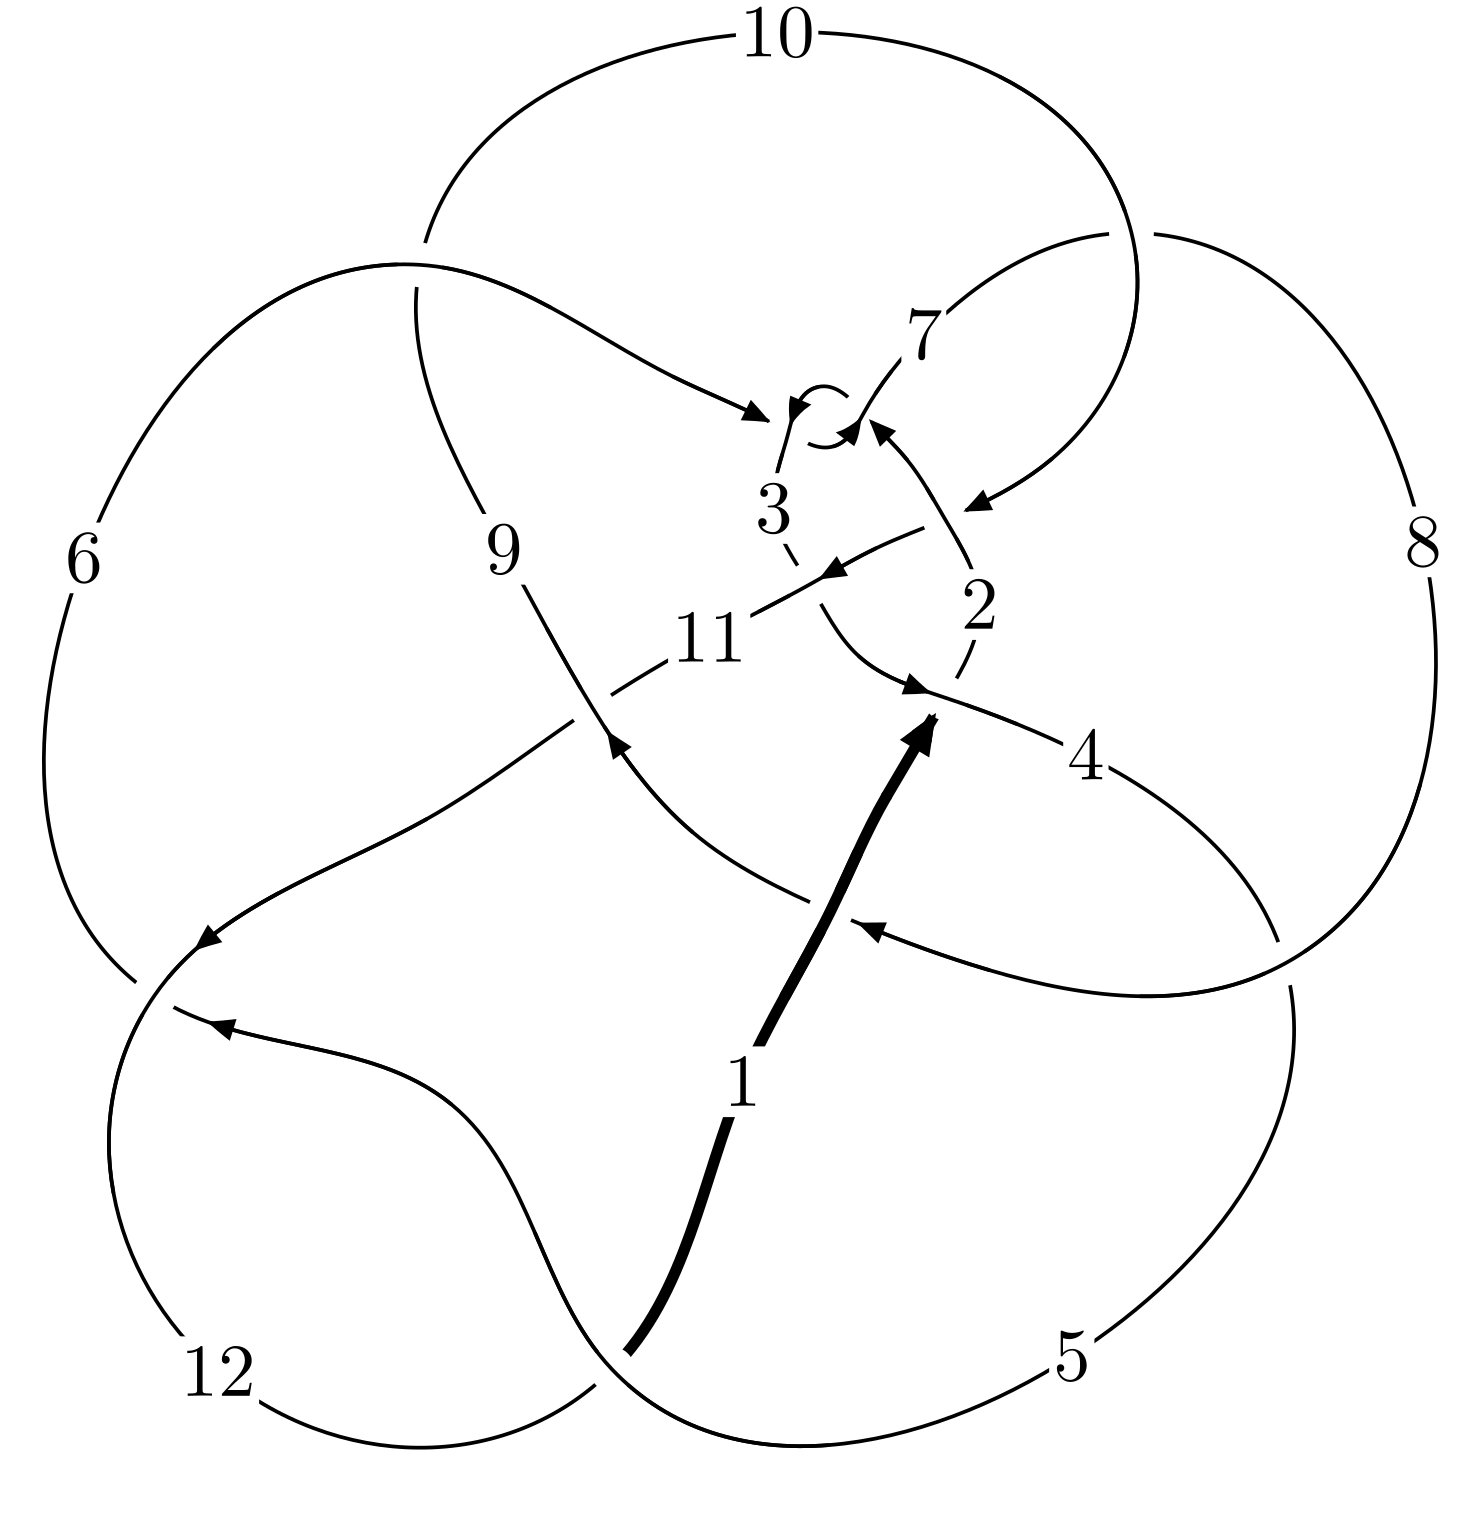
\includegraphics[width=112pt]{../../../GIT/diagram.site/Diagrams/png/1899_12a_1098.png}\\
\ \ \ A knot diagram\footnotemark}&
\allowdisplaybreaks
\textbf{Linearized knot diagam} \\
\cline{2-2}
 &
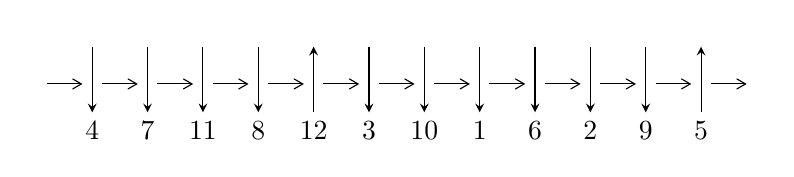
\begin{tikzpicture}[x=20pt, y=17pt]
	% nodes
	\node (C0) at (0, 0) {};
	\node (C1) at (1, 0) {};
	\node (C1U) at (1, +1) {};
	\node (C1D) at (1, -1) {4};

	\node (C2) at (2, 0) {};
	\node (C2U) at (2, +1) {};
	\node (C2D) at (2, -1) {7};

	\node (C3) at (3, 0) {};
	\node (C3U) at (3, +1) {};
	\node (C3D) at (3, -1) {11};

	\node (C4) at (4, 0) {};
	\node (C4U) at (4, +1) {};
	\node (C4D) at (4, -1) {8};

	\node (C5) at (5, 0) {};
	\node (C5U) at (5, +1) {};
	\node (C5D) at (5, -1) {12};

	\node (C6) at (6, 0) {};
	\node (C6U) at (6, +1) {};
	\node (C6D) at (6, -1) {3};

	\node (C7) at (7, 0) {};
	\node (C7U) at (7, +1) {};
	\node (C7D) at (7, -1) {10};

	\node (C8) at (8, 0) {};
	\node (C8U) at (8, +1) {};
	\node (C8D) at (8, -1) {1};

	\node (C9) at (9, 0) {};
	\node (C9U) at (9, +1) {};
	\node (C9D) at (9, -1) {6};

	\node (C10) at (10, 0) {};
	\node (C10U) at (10, +1) {};
	\node (C10D) at (10, -1) {2};

	\node (C11) at (11, 0) {};
	\node (C11U) at (11, +1) {};
	\node (C11D) at (11, -1) {9};

	\node (C12) at (12, 0) {};
	\node (C12U) at (12, +1) {};
	\node (C12D) at (12, -1) {5};
	\node (C13) at (13, 0) {};

	% arrows
	\draw[->,>={angle 60}]
	(C0) edge (C1) (C1) edge (C2) (C2) edge (C3) (C3) edge (C4) (C4) edge (C5) (C5) edge (C6) (C6) edge (C7) (C7) edge (C8) (C8) edge (C9) (C9) edge (C10) (C10) edge (C11) (C11) edge (C12) (C12) edge (C13) ;	\draw[->,>=stealth]
	(C1U) edge (C1D) (C2U) edge (C2D) (C3U) edge (C3D) (C4U) edge (C4D) (C5D) edge (C5U) (C6U) edge (C6D) (C7U) edge (C7D) (C8U) edge (C8D) (C9U) edge (C9D) (C10U) edge (C10D) (C11U) edge (C11D) (C12D) edge (C12U) ;
	\end{tikzpicture} \\
\hhline{~~} \\& 
\textbf{Solving Sequence} \\ \cline{2-2} 
 &
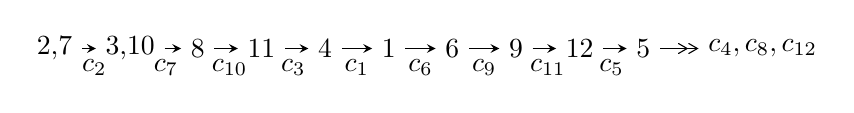
\begin{tikzpicture}[x=23pt, y=7pt]
	% node
	\node (A0) at (-1/8, 0) {2,7};
	\node (A1) at (17/16, 0) {3,10};
	\node (A2) at (17/8, 0) {8};
	\node (A3) at (25/8, 0) {11};
	\node (A4) at (33/8, 0) {4};
	\node (A5) at (41/8, 0) {1};
	\node (A6) at (49/8, 0) {6};
	\node (A7) at (57/8, 0) {9};
	\node (A8) at (65/8, 0) {12};
	\node (A9) at (73/8, 0) {5};
	\node (C1) at (1/2, -1) {$c_{2}$};
	\node (C2) at (13/8, -1) {$c_{7}$};
	\node (C3) at (21/8, -1) {$c_{10}$};
	\node (C4) at (29/8, -1) {$c_{3}$};
	\node (C5) at (37/8, -1) {$c_{1}$};
	\node (C6) at (45/8, -1) {$c_{6}$};
	\node (C7) at (53/8, -1) {$c_{9}$};
	\node (C8) at (61/8, -1) {$c_{11}$};
	\node (C9) at (69/8, -1) {$c_{5}$};
	\node (A10) at (11, 0) {$c_{4},c_{8},c_{12}$};

	% edge
	\draw[->,>=stealth]	
	(A0) edge (A1) (A1) edge (A2) (A2) edge (A3) (A3) edge (A4) (A4) edge (A5) (A5) edge (A6) (A6) edge (A7) (A7) edge (A8) (A8) edge (A9) ;
	\draw[->>,>={angle 60}]	
	(A9) edge (A10);
\end{tikzpicture} \\ 

\end{tabular} \\

\footnotetext{
The image of knot diagram is generated by the software ``\textbf{Draw programme}" developed by Andrew Bartholomew(\url{http://www.layer8.co.uk/maths/draw/index.htm\#Running-draw}), where we modified some parts for our purpose(\url{https://github.com/CATsTAILs/LinksPainter}).
}\phantom \\ \newline 
\centering \textbf{Ideals for irreducible components\footnotemark of $X_{\text{par}}$} 
 
\begin{align*}
I^u_{1}&=\langle 
1.26039\times10^{1096} u^{194}-5.54845\times10^{1096} u^{193}+\cdots+8.23984\times10^{1095} b+9.42064\times10^{1099},\\
\phantom{I^u_{1}}&\phantom{= \langle  }2.37059\times10^{1099} u^{194}-6.13693\times10^{1099} u^{193}+\cdots+4.63779\times10^{1099} a-5.55624\times10^{1103},\\
\phantom{I^u_{1}}&\phantom{= \langle  }u^{195}-4 u^{194}+\cdots+113416 u-11257\rangle \\
I^u_{2}&=\langle 
1.09077\times10^{50} u^{48}-2.47702\times10^{51} u^{47}+\cdots+9.36422\times10^{50} b+5.62660\times10^{51},\\
\phantom{I^u_{2}}&\phantom{= \langle  }-2.12833\times10^{51} u^{48}+2.10958\times10^{51} u^{47}+\cdots+2.34105\times10^{51} a-1.43194\times10^{51},\;u^{49}- u^{48}+\cdots+u-1\rangle \\
\\
\end{align*}
\raggedright * 2 irreducible components of $\dim_{\mathbb{C}}=0$, with total 244 representations.\\
\footnotetext{All coefficients of polynomials are rational numbers. But the coefficients are sometimes approximated in decimal forms when there is not enough margin.}
\newpage
\renewcommand{\arraystretch}{1}
\centering \section*{I. $I^u_{1}= \langle 1.26\times10^{1096} u^{194}-5.55\times10^{1096} u^{193}+\cdots+8.24\times10^{1095} b+9.42\times10^{1099},\;2.37\times10^{1099} u^{194}-6.14\times10^{1099} u^{193}+\cdots+4.64\times10^{1099} a-5.56\times10^{1103},\;u^{195}-4 u^{194}+\cdots+113416 u-11257 \rangle$}
\flushleft \textbf{(i) Arc colorings}\\
\begin{tabular}{m{7pt} m{180pt} m{7pt} m{180pt} }
\flushright $a_{2}=$&$\begin{pmatrix}1\\0\end{pmatrix}$ \\
\flushright $a_{7}=$&$\begin{pmatrix}0\\u\end{pmatrix}$ \\
\flushright $a_{3}=$&$\begin{pmatrix}1\\u^2\end{pmatrix}$ \\
\flushright $a_{10}=$&$\begin{pmatrix}-0.511146 u^{194}+1.32324 u^{193}+\cdots-111315. u+11980.3\\-1.52962 u^{194}+6.73368 u^{193}+\cdots+145905. u-11433.0\end{pmatrix}$ \\
\flushright $a_{8}=$&$\begin{pmatrix}-1.47117 u^{194}+4.65577 u^{193}+\cdots-211659. u+23522.7\\-0.673752 u^{194}+3.08530 u^{193}+\cdots+111463. u-9696.62\end{pmatrix}$ \\
\flushright $a_{11}=$&$\begin{pmatrix}1.01848 u^{194}-5.41044 u^{193}+\cdots-257220. u+23413.4\\-1.52962 u^{194}+6.73368 u^{193}+\cdots+145905. u-11433.0\end{pmatrix}$ \\
\flushright $a_{4}=$&$\begin{pmatrix}0.586225 u^{194}-1.53369 u^{193}+\cdots+165820. u-17237.5\\-1.34404 u^{194}+5.86482 u^{193}+\cdots+77525.5 u-5505.19\end{pmatrix}$ \\
\flushright $a_{1}=$&$\begin{pmatrix}0.151020 u^{194}-0.597552 u^{193}+\cdots+44952.6 u-4866.48\\0.439914 u^{194}-1.61276 u^{193}+\cdots-25671.4 u+1685.20\end{pmatrix}$ \\
\flushright $a_{6}=$&$\begin{pmatrix}u\\u^3+u\end{pmatrix}$ \\
\flushright $a_{9}=$&$\begin{pmatrix}0.120201 u^{194}-1.70426 u^{193}+\cdots-233869. u+22632.2\\-1.08301 u^{194}+4.59774 u^{193}+\cdots+87405.6 u-6433.53\end{pmatrix}$ \\
\flushright $a_{12}=$&$\begin{pmatrix}-0.394897 u^{194}+2.63210 u^{193}+\cdots+215956. u-21265.2\\-0.0681673 u^{194}+0.197496 u^{193}+\cdots-22256.9 u+2233.41\end{pmatrix}$ \\
\flushright $a_{5}=$&$\begin{pmatrix}1.97245 u^{194}-7.45707 u^{193}+\cdots-14130.9 u-2521.77\\-0.169214 u^{194}+0.611793 u^{193}+\cdots-22516.2 u+2913.54\end{pmatrix}$\\&\end{tabular}
\flushleft \textbf{(ii) Obstruction class $= -1$}\\~\\
\flushleft \textbf{(iii) Cusp Shapes $= -2.69583 u^{194}+0.189744 u^{193}+\cdots-1.88279\times10^{6} u+187667.$}\\~\\
\newpage\renewcommand{\arraystretch}{1}
\flushleft \textbf{(iv) u-Polynomials at the component}\newline \\
\begin{tabular}{m{50pt}|m{274pt}}
Crossings & \hspace{64pt}u-Polynomials at each crossing \\
\hline $$\begin{aligned}c_{1}\end{aligned}$$&$\begin{aligned}
&u^{195}-16 u^{194}+\cdots-2141 u+88
\end{aligned}$\\
\hline $$\begin{aligned}c_{2},c_{6}\end{aligned}$$&$\begin{aligned}
&u^{195}+4 u^{194}+\cdots+113416 u+11257
\end{aligned}$\\
\hline $$\begin{aligned}c_{3}\end{aligned}$$&$\begin{aligned}
&u^{195}-3 u^{194}+\cdots+217741 u+10918
\end{aligned}$\\
\hline $$\begin{aligned}c_{4}\end{aligned}$$&$\begin{aligned}
&u^{195}+4 u^{194}+\cdots+51821 u+2894
\end{aligned}$\\
\hline $$\begin{aligned}c_{5},c_{12}\end{aligned}$$&$\begin{aligned}
&u^{195}-3 u^{194}+\cdots+23431 u+1133
\end{aligned}$\\
\hline $$\begin{aligned}c_{7}\end{aligned}$$&$\begin{aligned}
&u^{195}+11 u^{194}+\cdots+218148168 u+31728989
\end{aligned}$\\
\hline $$\begin{aligned}c_{8}\end{aligned}$$&$\begin{aligned}
&2(2 u^{195}+7 u^{194}+\cdots-49 u+5)
\end{aligned}$\\
\hline $$\begin{aligned}c_{9}\end{aligned}$$&$\begin{aligned}
&2(2 u^{195}-9 u^{194}+\cdots-5.76855\times10^{7} u+4.42253\times10^{7})
\end{aligned}$\\
\hline $$\begin{aligned}c_{10}\end{aligned}$$&$\begin{aligned}
&2(2 u^{195}+25 u^{194}+\cdots+1.02982\times10^{7} u+574285)
\end{aligned}$\\
\hline $$\begin{aligned}c_{11}\end{aligned}$$&$\begin{aligned}
&u^{195}+8 u^{194}+\cdots+12939 u+1819
\end{aligned}$\\
\hline
\end{tabular}\\~\\
\newpage\renewcommand{\arraystretch}{1}
\flushleft \textbf{(v) Riley Polynomials at the component}\newline \\
\begin{tabular}{m{50pt}|m{274pt}}
Crossings & \hspace{64pt}Riley Polynomials at each crossing \\
\hline $$\begin{aligned}c_{1}\end{aligned}$$&$\begin{aligned}
&y^{195}+62 y^{194}+\cdots-185895 y-7744
\end{aligned}$\\
\hline $$\begin{aligned}c_{2},c_{6}\end{aligned}$$&$\begin{aligned}
&y^{195}+116 y^{194}+\cdots-6845116264 y-126720049
\end{aligned}$\\
\hline $$\begin{aligned}c_{3}\end{aligned}$$&$\begin{aligned}
&y^{195}+45 y^{194}+\cdots+993877489 y-119202724
\end{aligned}$\\
\hline $$\begin{aligned}c_{4}\end{aligned}$$&$\begin{aligned}
&y^{195}-28 y^{194}+\cdots+583712209 y-8375236
\end{aligned}$\\
\hline $$\begin{aligned}c_{5},c_{12}\end{aligned}$$&$\begin{aligned}
&y^{195}+147 y^{194}+\cdots+20891003 y-1283689
\end{aligned}$\\
\hline $$\begin{aligned}c_{7}\end{aligned}$$&$\begin{aligned}
&y^{195}+9 y^{194}+\cdots-60843014639712268 y-1006728742962121
\end{aligned}$\\
\hline $$\begin{aligned}c_{8}\end{aligned}$$&$\begin{aligned}
&4(4 y^{195}-73 y^{194}+\cdots+211 y-25)
\end{aligned}$\\
\hline $$\begin{aligned}c_{9}\end{aligned}$$&$\begin{aligned}
&4\\
&\cdot(4 y^{195}-261 y^{194}+\cdots+8953659438498701 y-1955874418122361)
\end{aligned}$\\
\hline $$\begin{aligned}c_{10}\end{aligned}$$&$\begin{aligned}
&4(4 y^{195}+159 y^{194}+\cdots+1.74880\times10^{13} y-3.29803\times10^{11})
\end{aligned}$\\
\hline $$\begin{aligned}c_{11}\end{aligned}$$&$\begin{aligned}
&y^{195}-42 y^{194}+\cdots-2071600293 y-3308761
\end{aligned}$\\
\hline
\end{tabular}\\~\\
\newpage\flushleft \textbf{(vi) Complex Volumes and Cusp Shapes}
$$\begin{array}{c|c|c}  
\text{Solutions to }I^u_{1}& \I (\text{vol} + \sqrt{-1}CS) & \text{Cusp shape}\\
 \hline 
\begin{aligned}
u &= -0.229847 + 0.974311 I \\
a &= \phantom{-}0.30308 + 1.40779 I \\
b &= \phantom{-}0.55537 - 1.33039 I\end{aligned}
 & -1.80544 + 4.08060 I & \phantom{-0.000000 } 0 \\ \hline\begin{aligned}
u &= -0.229847 - 0.974311 I \\
a &= \phantom{-}0.30308 - 1.40779 I \\
b &= \phantom{-}0.55537 + 1.33039 I\end{aligned}
 & -1.80544 - 4.08060 I & \phantom{-0.000000 } 0 \\ \hline\begin{aligned}
u &= -0.635598 + 0.766858 I \\
a &= \phantom{-}0.175078 - 0.073876 I \\
b &= -0.615392 - 1.058350 I\end{aligned}
 & -4.27809 - 4.36087 I & \phantom{-0.000000 } 0 \\ \hline\begin{aligned}
u &= -0.635598 - 0.766858 I \\
a &= \phantom{-}0.175078 + 0.073876 I \\
b &= -0.615392 + 1.058350 I\end{aligned}
 & -4.27809 + 4.36087 I & \phantom{-0.000000 } 0 \\ \hline\begin{aligned}
u &= -0.213608 + 0.982090 I \\
a &= -0.284603 + 0.247759 I \\
b &= -1.11742 - 1.69158 I\end{aligned}
 & -2.58548 + 5.44227 I & \phantom{-0.000000 } 0 \\ \hline\begin{aligned}
u &= -0.213608 - 0.982090 I \\
a &= -0.284603 - 0.247759 I \\
b &= -1.11742 + 1.69158 I\end{aligned}
 & -2.58548 - 5.44227 I & \phantom{-0.000000 } 0 \\ \hline\begin{aligned}
u &= \phantom{-}0.044460 + 1.009420 I \\
a &= -1.76948 + 0.19269 I \\
b &= -0.775797 - 0.693267 I\end{aligned}
 & \phantom{-}1.66899 - 5.60569 I & \phantom{-0.000000 } 0 \\ \hline\begin{aligned}
u &= \phantom{-}0.044460 - 1.009420 I \\
a &= -1.76948 - 0.19269 I \\
b &= -0.775797 + 0.693267 I\end{aligned}
 & \phantom{-}1.66899 + 5.60569 I & \phantom{-0.000000 } 0 \\ \hline\begin{aligned}
u &= \phantom{-}0.081752 + 1.008600 I \\
a &= \phantom{-}1.42458 + 1.07381 I \\
b &= \phantom{-}0.352065 - 0.913459 I\end{aligned}
 & \phantom{-}3.96016 + 0.37043 I & \phantom{-0.000000 } 0 \\ \hline\begin{aligned}
u &= \phantom{-}0.081752 - 1.008600 I \\
a &= \phantom{-}1.42458 - 1.07381 I \\
b &= \phantom{-}0.352065 + 0.913459 I\end{aligned}
 & \phantom{-}3.96016 - 0.37043 I & \phantom{-0.000000 } 0\\
 \hline 
 \end{array}$$\newpage$$\begin{array}{c|c|c}  
\text{Solutions to }I^u_{1}& \I (\text{vol} + \sqrt{-1}CS) & \text{Cusp shape}\\
 \hline 
\begin{aligned}
u &= -0.340357 + 0.927028 I \\
a &= \phantom{-}0.99354 - 1.55193 I \\
b &= \phantom{-}0.153232 - 0.041064 I\end{aligned}
 & -3.83954 + 6.18863 I & \phantom{-0.000000 } 0 \\ \hline\begin{aligned}
u &= -0.340357 - 0.927028 I \\
a &= \phantom{-}0.99354 + 1.55193 I \\
b &= \phantom{-}0.153232 + 0.041064 I\end{aligned}
 & -3.83954 - 6.18863 I & \phantom{-0.000000 } 0 \\ \hline\begin{aligned}
u &= -0.949863 + 0.352493 I \\
a &= \phantom{-}0.331428 + 0.731583 I \\
b &= -0.145725 + 0.629283 I\end{aligned}
 & -1.59057 + 0.63800 I & \phantom{-0.000000 } 0 \\ \hline\begin{aligned}
u &= -0.949863 - 0.352493 I \\
a &= \phantom{-}0.331428 - 0.731583 I \\
b &= -0.145725 - 0.629283 I\end{aligned}
 & -1.59057 - 0.63800 I & \phantom{-0.000000 } 0 \\ \hline\begin{aligned}
u &= \phantom{-}0.985579 + 0.005049 I \\
a &= \phantom{-}0.820488 + 0.440894 I \\
b &= \phantom{-}0.875081 + 0.811497 I\end{aligned}
 & -3.41252 - 2.70500 I & \phantom{-0.000000 } 0 \\ \hline\begin{aligned}
u &= \phantom{-}0.985579 - 0.005049 I \\
a &= \phantom{-}0.820488 - 0.440894 I \\
b &= \phantom{-}0.875081 - 0.811497 I\end{aligned}
 & -3.41252 + 2.70500 I & \phantom{-0.000000 } 0 \\ \hline\begin{aligned}
u &= -0.279959 + 0.939793 I \\
a &= -0.482096 - 0.337591 I \\
b &= -1.94105 - 0.40614 I\end{aligned}
 & \phantom{-}1.84118 + 6.62127 I & \phantom{-0.000000 } 0 \\ \hline\begin{aligned}
u &= -0.279959 - 0.939793 I \\
a &= -0.482096 + 0.337591 I \\
b &= -1.94105 + 0.40614 I\end{aligned}
 & \phantom{-}1.84118 - 6.62127 I & \phantom{-0.000000 } 0 \\ \hline\begin{aligned}
u &= -0.956595 + 0.206169 I \\
a &= \phantom{-}0.488973 + 1.095580 I \\
b &= \phantom{-}0.690719 + 0.974454 I\end{aligned}
 & -0.50653 - 4.70693 I & \phantom{-0.000000 } 0 \\ \hline\begin{aligned}
u &= -0.956595 - 0.206169 I \\
a &= \phantom{-}0.488973 - 1.095580 I \\
b &= \phantom{-}0.690719 - 0.974454 I\end{aligned}
 & -0.50653 + 4.70693 I & \phantom{-0.000000 } 0\\
 \hline 
 \end{array}$$\newpage$$\begin{array}{c|c|c}  
\text{Solutions to }I^u_{1}& \I (\text{vol} + \sqrt{-1}CS) & \text{Cusp shape}\\
 \hline 
\begin{aligned}
u &= \phantom{-}0.215211 + 1.000710 I \\
a &= -1.101110 + 0.746345 I \\
b &= -1.71977 + 0.31148 I\end{aligned}
 & -2.79903 - 1.55519 I & \phantom{-0.000000 } 0 \\ \hline\begin{aligned}
u &= \phantom{-}0.215211 - 1.000710 I \\
a &= -1.101110 - 0.746345 I \\
b &= -1.71977 - 0.31148 I\end{aligned}
 & -2.79903 + 1.55519 I & \phantom{-0.000000 } 0 \\ \hline\begin{aligned}
u &= -0.151109 + 1.016340 I \\
a &= \phantom{-}0.89528 - 1.95590 I \\
b &= -0.218993 + 0.567699 I\end{aligned}
 & \phantom{-}3.11920 + 5.88513 I & \phantom{-0.000000 } 0 \\ \hline\begin{aligned}
u &= -0.151109 - 1.016340 I \\
a &= \phantom{-}0.89528 + 1.95590 I \\
b &= -0.218993 - 0.567699 I\end{aligned}
 & \phantom{-}3.11920 - 5.88513 I & \phantom{-0.000000 } 0 \\ \hline\begin{aligned}
u &= \phantom{-}0.842804 + 0.455707 I \\
a &= -0.344177 + 1.272260 I \\
b &= -0.84360 + 1.17309 I\end{aligned}
 & -2.98538 + 5.10576 I & \phantom{-0.000000 } 0 \\ \hline\begin{aligned}
u &= \phantom{-}0.842804 - 0.455707 I \\
a &= -0.344177 - 1.272260 I \\
b &= -0.84360 - 1.17309 I\end{aligned}
 & -2.98538 - 5.10576 I & \phantom{-0.000000 } 0 \\ \hline\begin{aligned}
u &= -0.998905 + 0.299241 I \\
a &= \phantom{-}0.700680 - 1.097540 I \\
b &= \phantom{-}0.581880 - 0.818240 I\end{aligned}
 & -0.77731 + 7.34371 I & \phantom{-0.000000 } 0 \\ \hline\begin{aligned}
u &= -0.998905 - 0.299241 I \\
a &= \phantom{-}0.700680 + 1.097540 I \\
b &= \phantom{-}0.581880 + 0.818240 I\end{aligned}
 & -0.77731 - 7.34371 I & \phantom{-0.000000 } 0 \\ \hline\begin{aligned}
u &= \phantom{-}0.463041 + 0.837478 I \\
a &= \phantom{-}1.32810 + 0.70895 I \\
b &= -0.040835 + 1.061810 I\end{aligned}
 & \phantom{-}0.80944 + 4.01559 I & \phantom{-0.000000 } 0 \\ \hline\begin{aligned}
u &= \phantom{-}0.463041 - 0.837478 I \\
a &= \phantom{-}1.32810 - 0.70895 I \\
b &= -0.040835 - 1.061810 I\end{aligned}
 & \phantom{-}0.80944 - 4.01559 I & \phantom{-0.000000 } 0\\
 \hline 
 \end{array}$$\newpage$$\begin{array}{c|c|c}  
\text{Solutions to }I^u_{1}& \I (\text{vol} + \sqrt{-1}CS) & \text{Cusp shape}\\
 \hline 
\begin{aligned}
u &= \phantom{-}0.005129 + 0.954379 I \\
a &= -1.41357 - 0.26872 I \\
b &= -0.347241 + 0.838567 I\end{aligned}
 & \phantom{-}3.55479 - 0.87622 I & \phantom{-0.000000 } 0 \\ \hline\begin{aligned}
u &= \phantom{-}0.005129 - 0.954379 I \\
a &= -1.41357 + 0.26872 I \\
b &= -0.347241 - 0.838567 I\end{aligned}
 & \phantom{-}3.55479 + 0.87622 I & \phantom{-0.000000 } 0 \\ \hline\begin{aligned}
u &= -0.910905 + 0.261615 I \\
a &= \phantom{-}1.208150 + 0.557838 I \\
b &= \phantom{-}0.843854 + 0.550938 I\end{aligned}
 & -5.82793 - 1.97974 I & \phantom{-0.000000 } 0 \\ \hline\begin{aligned}
u &= -0.910905 - 0.261615 I \\
a &= \phantom{-}1.208150 - 0.557838 I \\
b &= \phantom{-}0.843854 - 0.550938 I\end{aligned}
 & -5.82793 + 1.97974 I & \phantom{-0.000000 } 0 \\ \hline\begin{aligned}
u &= -0.352869 + 0.999237 I \\
a &= \phantom{-}1.309980 + 0.124605 I \\
b &= \phantom{-}1.123490 - 0.168123 I\end{aligned}
 & -2.66413 + 5.29690 I & \phantom{-0.000000 } 0 \\ \hline\begin{aligned}
u &= -0.352869 - 0.999237 I \\
a &= \phantom{-}1.309980 - 0.124605 I \\
b &= \phantom{-}1.123490 + 0.168123 I\end{aligned}
 & -2.66413 - 5.29690 I & \phantom{-0.000000 } 0 \\ \hline\begin{aligned}
u &= \phantom{-}0.326697 + 1.014140 I \\
a &= \phantom{-}0.561261 - 0.508035 I \\
b &= \phantom{-}1.94125 - 0.64929 I\end{aligned}
 & -2.65706 - 12.16010 I & \phantom{-0.000000 } 0 \\ \hline\begin{aligned}
u &= \phantom{-}0.326697 - 1.014140 I \\
a &= \phantom{-}0.561261 + 0.508035 I \\
b &= \phantom{-}1.94125 + 0.64929 I\end{aligned}
 & -2.65706 + 12.16010 I & \phantom{-0.000000 } 0 \\ \hline\begin{aligned}
u &= \phantom{-}0.926967 + 0.113254 I \\
a &= -0.184218 + 0.754293 I \\
b &= \phantom{-}0.311515 + 0.714463 I\end{aligned}
 & -0.528284 - 0.958478 I & \phantom{-0.000000 } 0 \\ \hline\begin{aligned}
u &= \phantom{-}0.926967 - 0.113254 I \\
a &= -0.184218 - 0.754293 I \\
b &= \phantom{-}0.311515 - 0.714463 I\end{aligned}
 & -0.528284 + 0.958478 I & \phantom{-0.000000 } 0\\
 \hline 
 \end{array}$$\newpage$$\begin{array}{c|c|c}  
\text{Solutions to }I^u_{1}& \I (\text{vol} + \sqrt{-1}CS) & \text{Cusp shape}\\
 \hline 
\begin{aligned}
u &= -0.193536 + 1.054740 I \\
a &= \phantom{-}0.032676 + 0.585986 I \\
b &= \phantom{-}1.71292 + 1.77353 I\end{aligned}
 & -0.939947 - 0.000035 I & \phantom{-0.000000 } 0 \\ \hline\begin{aligned}
u &= -0.193536 - 1.054740 I \\
a &= \phantom{-}0.032676 - 0.585986 I \\
b &= \phantom{-}1.71292 - 1.77353 I\end{aligned}
 & -0.939947 + 0.000035 I & \phantom{-0.000000 } 0 \\ \hline\begin{aligned}
u &= \phantom{-}0.334551 + 1.021810 I \\
a &= -0.486973 - 0.143961 I \\
b &= -0.697169 + 0.461883 I\end{aligned}
 & \phantom{-}1.55837 - 2.94938 I & \phantom{-0.000000 } 0 \\ \hline\begin{aligned}
u &= \phantom{-}0.334551 - 1.021810 I \\
a &= -0.486973 + 0.143961 I \\
b &= -0.697169 - 0.461883 I\end{aligned}
 & \phantom{-}1.55837 + 2.94938 I & \phantom{-0.000000 } 0 \\ \hline\begin{aligned}
u &= \phantom{-}0.623008 + 0.662516 I \\
a &= \phantom{-}0.100188 - 0.348881 I \\
b &= \phantom{-}0.984468 - 0.203862 I\end{aligned}
 & -2.15925 - 1.04139 I & \phantom{-0.000000 } 0 \\ \hline\begin{aligned}
u &= \phantom{-}0.623008 - 0.662516 I \\
a &= \phantom{-}0.100188 + 0.348881 I \\
b &= \phantom{-}0.984468 + 0.203862 I\end{aligned}
 & -2.15925 + 1.04139 I & \phantom{-0.000000 } 0 \\ \hline\begin{aligned}
u &= \phantom{-}0.188072 + 0.885745 I \\
a &= \phantom{-}0.18189 - 3.35363 I \\
b &= \phantom{-}0.445617 + 0.277728 I\end{aligned}
 & -3.11330 - 10.34180 I & \phantom{-0.000000 } 0 \\ \hline\begin{aligned}
u &= \phantom{-}0.188072 - 0.885745 I \\
a &= \phantom{-}0.18189 + 3.35363 I \\
b &= \phantom{-}0.445617 - 0.277728 I\end{aligned}
 & -3.11330 + 10.34180 I & \phantom{-0.000000 } 0 \\ \hline\begin{aligned}
u &= -0.135708 + 0.881152 I \\
a &= \phantom{-}0.817279 + 0.782255 I \\
b &= \phantom{-}1.55399 - 0.16843 I\end{aligned}
 & -0.893570 + 0.937338 I & \phantom{-0.000000 } 0 \\ \hline\begin{aligned}
u &= -0.135708 - 0.881152 I \\
a &= \phantom{-}0.817279 - 0.782255 I \\
b &= \phantom{-}1.55399 + 0.16843 I\end{aligned}
 & -0.893570 - 0.937338 I & \phantom{-0.000000 } 0\\
 \hline 
 \end{array}$$\newpage$$\begin{array}{c|c|c}  
\text{Solutions to }I^u_{1}& \I (\text{vol} + \sqrt{-1}CS) & \text{Cusp shape}\\
 \hline 
\begin{aligned}
u &= \phantom{-}1.109500 + 0.139095 I \\
a &= -0.733889 + 1.065730 I \\
b &= -0.714813 + 0.933276 I\end{aligned}
 & -4.29066 + 5.83447 I & \phantom{-0.000000 } 0 \\ \hline\begin{aligned}
u &= \phantom{-}1.109500 - 0.139095 I \\
a &= -0.733889 - 1.065730 I \\
b &= -0.714813 - 0.933276 I\end{aligned}
 & -4.29066 - 5.83447 I & \phantom{-0.000000 } 0 \\ \hline\begin{aligned}
u &= -1.119570 + 0.106898 I \\
a &= -0.617179 - 0.802897 I \\
b &= -0.756292 - 0.934165 I\end{aligned}
 & \phantom{-}0.78469 - 9.60406 I & \phantom{-0.000000 } 0 \\ \hline\begin{aligned}
u &= -1.119570 - 0.106898 I \\
a &= -0.617179 + 0.802897 I \\
b &= -0.756292 + 0.934165 I\end{aligned}
 & \phantom{-}0.78469 + 9.60406 I & \phantom{-0.000000 } 0 \\ \hline\begin{aligned}
u &= \phantom{-}0.846829 + 0.209085 I \\
a &= -0.731495 + 0.502899 I \\
b &= -0.530183 - 0.112186 I\end{aligned}
 & -1.33087 - 0.72319 I & \phantom{-0.000000 } 0 \\ \hline\begin{aligned}
u &= \phantom{-}0.846829 - 0.209085 I \\
a &= -0.731495 - 0.502899 I \\
b &= -0.530183 + 0.112186 I\end{aligned}
 & -1.33087 + 0.72319 I & \phantom{-0.000000 } 0 \\ \hline\begin{aligned}
u &= \phantom{-}0.018353 + 0.866884 I \\
a &= \phantom{-}0.556628 + 0.523527 I \\
b &= \phantom{-}1.70481 - 0.51962 I\end{aligned}
 & -0.751573 + 0.863225 I & \phantom{-0.000000 } 0 \\ \hline\begin{aligned}
u &= \phantom{-}0.018353 - 0.866884 I \\
a &= \phantom{-}0.556628 - 0.523527 I \\
b &= \phantom{-}1.70481 + 0.51962 I\end{aligned}
 & -0.751573 - 0.863225 I & \phantom{-0.000000 } 0 \\ \hline\begin{aligned}
u &= -0.679044 + 0.533411 I \\
a &= \phantom{-}0.47379 + 1.50522 I \\
b &= \phantom{-}0.842970 + 0.400250 I\end{aligned}
 & -4.49809 - 1.53846 I & \phantom{-0.000000 } 0 \\ \hline\begin{aligned}
u &= -0.679044 - 0.533411 I \\
a &= \phantom{-}0.47379 - 1.50522 I \\
b &= \phantom{-}0.842970 - 0.400250 I\end{aligned}
 & -4.49809 + 1.53846 I & \phantom{-0.000000 } 0\\
 \hline 
 \end{array}$$\newpage$$\begin{array}{c|c|c}  
\text{Solutions to }I^u_{1}& \I (\text{vol} + \sqrt{-1}CS) & \text{Cusp shape}\\
 \hline 
\begin{aligned}
u &= -1.083240 + 0.346377 I \\
a &= \phantom{-}0.191066 + 0.952447 I \\
b &= \phantom{-}0.513660 + 1.092630 I\end{aligned}
 & -0.76440 - 5.39606 I & \phantom{-0.000000 } 0 \\ \hline\begin{aligned}
u &= -1.083240 - 0.346377 I \\
a &= \phantom{-}0.191066 - 0.952447 I \\
b &= \phantom{-}0.513660 - 1.092630 I\end{aligned}
 & -0.76440 + 5.39606 I & \phantom{-0.000000 } 0 \\ \hline\begin{aligned}
u &= \phantom{-}0.442759 + 0.739069 I \\
a &= -1.21870 + 1.35018 I \\
b &= -1.334780 - 0.103594 I\end{aligned}
 & -5.38476 - 1.87072 I & \phantom{-0.000000 } 0 \\ \hline\begin{aligned}
u &= \phantom{-}0.442759 - 0.739069 I \\
a &= -1.21870 - 1.35018 I \\
b &= -1.334780 + 0.103594 I\end{aligned}
 & -5.38476 + 1.87072 I & \phantom{-0.000000 } 0 \\ \hline\begin{aligned}
u &= \phantom{-}1.136230 + 0.150504 I \\
a &= \phantom{-}0.678927 - 0.928671 I \\
b &= \phantom{-}0.784452 - 1.006980 I\end{aligned}
 & -3.9314 + 15.3997 I & \phantom{-0.000000 } 0 \\ \hline\begin{aligned}
u &= \phantom{-}1.136230 - 0.150504 I \\
a &= \phantom{-}0.678927 + 0.928671 I \\
b &= \phantom{-}0.784452 + 1.006980 I\end{aligned}
 & -3.9314 - 15.3997 I & \phantom{-0.000000 } 0 \\ \hline\begin{aligned}
u &= -0.153559 + 0.829785 I \\
a &= \phantom{-}0.56388 + 1.32275 I \\
b &= \phantom{-}1.27739 - 0.74715 I\end{aligned}
 & -0.980231 + 0.971067 I & \phantom{-0.000000 } 0 \\ \hline\begin{aligned}
u &= -0.153559 - 0.829785 I \\
a &= \phantom{-}0.56388 - 1.32275 I \\
b &= \phantom{-}1.27739 + 0.74715 I\end{aligned}
 & -0.980231 - 0.971067 I & \phantom{-0.000000 } 0 \\ \hline\begin{aligned}
u &= \phantom{-}0.307891 + 0.782104 I \\
a &= \phantom{-}2.23721 - 0.81181 I \\
b &= \phantom{-}1.031530 - 0.280647 I\end{aligned}
 & -3.18370 + 7.94529 I & \phantom{-0.000000 } 0 \\ \hline\begin{aligned}
u &= \phantom{-}0.307891 - 0.782104 I \\
a &= \phantom{-}2.23721 + 0.81181 I \\
b &= \phantom{-}1.031530 + 0.280647 I\end{aligned}
 & -3.18370 - 7.94529 I & \phantom{-0.000000 } 0\\
 \hline 
 \end{array}$$\newpage$$\begin{array}{c|c|c}  
\text{Solutions to }I^u_{1}& \I (\text{vol} + \sqrt{-1}CS) & \text{Cusp shape}\\
 \hline 
\begin{aligned}
u &= \phantom{-}0.367754 + 0.750622 I \\
a &= \phantom{-}0.619310 - 0.632085 I \\
b &= \phantom{-}0.103268 + 1.395740 I\end{aligned}
 & \phantom{-}0.21899 - 3.47149 I & \phantom{-0.000000 } 0 \\ \hline\begin{aligned}
u &= \phantom{-}0.367754 - 0.750622 I \\
a &= \phantom{-}0.619310 + 0.632085 I \\
b &= \phantom{-}0.103268 - 1.395740 I\end{aligned}
 & \phantom{-}0.21899 + 3.47149 I & \phantom{-0.000000 } 0 \\ \hline\begin{aligned}
u &= \phantom{-}0.449827 + 0.704123 I \\
a &= -1.49036 + 0.95298 I \\
b &= -1.184490 + 0.057036 I\end{aligned}
 & -5.39959 - 1.93014 I & \phantom{-0.000000 } 0 \\ \hline\begin{aligned}
u &= \phantom{-}0.449827 - 0.704123 I \\
a &= -1.49036 - 0.95298 I \\
b &= -1.184490 - 0.057036 I\end{aligned}
 & -5.39959 + 1.93014 I & \phantom{-0.000000 } 0 \\ \hline\begin{aligned}
u &= \phantom{-}0.388291 + 0.733947 I \\
a &= -1.11660 + 1.74454 I \\
b &= -0.845393 - 0.215975 I\end{aligned}
 & -5.34851 - 1.73934 I & \phantom{-0.000000 } 0 \\ \hline\begin{aligned}
u &= \phantom{-}0.388291 - 0.733947 I \\
a &= -1.11660 - 1.74454 I \\
b &= -0.845393 + 0.215975 I\end{aligned}
 & -5.34851 + 1.73934 I & \phantom{-0.000000 } 0 \\ \hline\begin{aligned}
u &= -0.165308 + 0.810412 I \\
a &= \phantom{-}0.56082 + 1.75127 I \\
b &= \phantom{-}0.882583 - 0.457074 I\end{aligned}
 & -1.02632 + 0.98406 I & \phantom{-0.000000 } 0 \\ \hline\begin{aligned}
u &= -0.165308 - 0.810412 I \\
a &= \phantom{-}0.56082 - 1.75127 I \\
b &= \phantom{-}0.882583 + 0.457074 I\end{aligned}
 & -1.02632 - 0.98406 I & \phantom{-0.000000 } 0 \\ \hline\begin{aligned}
u &= \phantom{-}0.510817 + 0.641566 I \\
a &= -1.25258 - 0.84716 I \\
b &= -0.685795 - 0.555487 I\end{aligned}
 & \phantom{-}1.66372 - 4.31307 I & \phantom{-0.000000 } 0 \\ \hline\begin{aligned}
u &= \phantom{-}0.510817 - 0.641566 I \\
a &= -1.25258 + 0.84716 I \\
b &= -0.685795 + 0.555487 I\end{aligned}
 & \phantom{-}1.66372 + 4.31307 I & \phantom{-0.000000 } 0\\
 \hline 
 \end{array}$$\newpage$$\begin{array}{c|c|c}  
\text{Solutions to }I^u_{1}& \I (\text{vol} + \sqrt{-1}CS) & \text{Cusp shape}\\
 \hline 
\begin{aligned}
u &= \phantom{-}1.178310 + 0.184999 I \\
a &= -0.332329 + 0.562029 I \\
b &= -0.395717 + 0.845977 I\end{aligned}
 & \phantom{-}0.08757 + 1.83094 I & \phantom{-0.000000 } 0 \\ \hline\begin{aligned}
u &= \phantom{-}1.178310 - 0.184999 I \\
a &= -0.332329 - 0.562029 I \\
b &= -0.395717 - 0.845977 I\end{aligned}
 & \phantom{-}0.08757 - 1.83094 I & \phantom{-0.000000 } 0 \\ \hline\begin{aligned}
u &= -0.372361 + 1.149840 I \\
a &= -0.878604 + 0.187577 I \\
b &= -0.153649 + 0.984248 I\end{aligned}
 & \phantom{-}4.10607 - 0.82015 I & \phantom{-0.000000 } 0 \\ \hline\begin{aligned}
u &= -0.372361 - 1.149840 I \\
a &= -0.878604 - 0.187577 I \\
b &= -0.153649 - 0.984248 I\end{aligned}
 & \phantom{-}4.10607 + 0.82015 I & \phantom{-0.000000 } 0 \\ \hline\begin{aligned}
u &= -0.506388 + 1.097430 I \\
a &= \phantom{-}1.324170 + 0.324307 I \\
b &= \phantom{-}1.048280 - 0.866838 I\end{aligned}
 & -2.63620 + 6.15137 I & \phantom{-0.000000 } 0 \\ \hline\begin{aligned}
u &= -0.506388 - 1.097430 I \\
a &= \phantom{-}1.324170 - 0.324307 I \\
b &= \phantom{-}1.048280 + 0.866838 I\end{aligned}
 & -2.63620 - 6.15137 I & \phantom{-0.000000 } 0 \\ \hline\begin{aligned}
u &= -0.210718 + 1.200420 I \\
a &= -1.93286 - 0.95517 I \\
b &= -0.302380 + 0.548108 I\end{aligned}
 & -0.11642 + 10.43800 I & \phantom{-0.000000 } 0 \\ \hline\begin{aligned}
u &= -0.210718 - 1.200420 I \\
a &= -1.93286 + 0.95517 I \\
b &= -0.302380 - 0.548108 I\end{aligned}
 & -0.11642 - 10.43800 I & \phantom{-0.000000 } 0 \\ \hline\begin{aligned}
u &= \phantom{-}0.137406 + 0.761054 I \\
a &= \phantom{-}0.06117 + 2.33645 I \\
b &= -1.030270 - 0.538505 I\end{aligned}
 & -3.73260 - 0.24421 I & \phantom{-0.000000 } 0 \\ \hline\begin{aligned}
u &= \phantom{-}0.137406 - 0.761054 I \\
a &= \phantom{-}0.06117 - 2.33645 I \\
b &= -1.030270 + 0.538505 I\end{aligned}
 & -3.73260 + 0.24421 I & \phantom{-0.000000 } 0\\
 \hline 
 \end{array}$$\newpage$$\begin{array}{c|c|c}  
\text{Solutions to }I^u_{1}& \I (\text{vol} + \sqrt{-1}CS) & \text{Cusp shape}\\
 \hline 
\begin{aligned}
u &= -0.479556 + 0.605344 I \\
a &= -1.153710 - 0.634733 I \\
b &= -0.004544 + 1.319820 I\end{aligned}
 & -4.64115 + 8.81274 I & \phantom{-0.000000 } 0 \\ \hline\begin{aligned}
u &= -0.479556 - 0.605344 I \\
a &= -1.153710 + 0.634733 I \\
b &= -0.004544 - 1.319820 I\end{aligned}
 & -4.64115 - 8.81274 I & \phantom{-0.000000 } 0 \\ \hline\begin{aligned}
u &= \phantom{-}0.299411 + 1.236170 I \\
a &= -0.748937 + 0.304351 I \\
b &= -1.07207 - 1.58322 I\end{aligned}
 & \phantom{-}6.31344 - 6.96124 I & \phantom{-0.000000 } 0 \\ \hline\begin{aligned}
u &= \phantom{-}0.299411 - 1.236170 I \\
a &= -0.748937 - 0.304351 I \\
b &= -1.07207 + 1.58322 I\end{aligned}
 & \phantom{-}6.31344 + 6.96124 I & \phantom{-0.000000 } 0 \\ \hline\begin{aligned}
u &= -0.052808 + 1.271950 I \\
a &= \phantom{-}0.278427 + 0.256074 I \\
b &= \phantom{-}0.906983 - 0.694726 I\end{aligned}
 & \phantom{-}0.431813 - 1.106830 I & \phantom{-0.000000 } 0 \\ \hline\begin{aligned}
u &= -0.052808 - 1.271950 I \\
a &= \phantom{-}0.278427 - 0.256074 I \\
b &= \phantom{-}0.906983 + 0.694726 I\end{aligned}
 & \phantom{-}0.431813 + 1.106830 I & \phantom{-0.000000 } 0 \\ \hline\begin{aligned}
u &= \phantom{-}0.354885 + 1.224060 I \\
a &= \phantom{-}1.086860 - 0.149759 I \\
b &= \phantom{-}0.87940 + 1.63490 I\end{aligned}
 & \phantom{-}4.45659 + 0.15218 I & \phantom{-0.000000 } 0 \\ \hline\begin{aligned}
u &= \phantom{-}0.354885 - 1.224060 I \\
a &= \phantom{-}1.086860 + 0.149759 I \\
b &= \phantom{-}0.87940 - 1.63490 I\end{aligned}
 & \phantom{-}4.45659 - 0.15218 I & \phantom{-0.000000 } 0 \\ \hline\begin{aligned}
u &= \phantom{-}0.633338 + 0.350421 I \\
a &= \phantom{-}1.379980 - 0.182928 I \\
b &= \phantom{-}0.817694 + 0.991932 I\end{aligned}
 & -2.86630 - 3.64019 I & \phantom{-0.000000 } 0 \\ \hline\begin{aligned}
u &= \phantom{-}0.633338 - 0.350421 I \\
a &= \phantom{-}1.379980 + 0.182928 I \\
b &= \phantom{-}0.817694 - 0.991932 I\end{aligned}
 & -2.86630 + 3.64019 I & \phantom{-0.000000 } 0\\
 \hline 
 \end{array}$$\newpage$$\begin{array}{c|c|c}  
\text{Solutions to }I^u_{1}& \I (\text{vol} + \sqrt{-1}CS) & \text{Cusp shape}\\
 \hline 
\begin{aligned}
u &= \phantom{-}0.577370 + 1.140060 I \\
a &= -1.42478 + 0.29961 I \\
b &= -0.92725 - 1.54153 I\end{aligned}
 & -0.80504 - 10.41690 I & \phantom{-0.000000 } 0 \\ \hline\begin{aligned}
u &= \phantom{-}0.577370 - 1.140060 I \\
a &= -1.42478 - 0.29961 I \\
b &= -0.92725 + 1.54153 I\end{aligned}
 & -0.80504 + 10.41690 I & \phantom{-0.000000 } 0 \\ \hline\begin{aligned}
u &= -0.368101 + 1.226320 I \\
a &= -1.080950 - 0.415193 I \\
b &= -0.89686 + 1.37051 I\end{aligned}
 & \phantom{-}7.49769 + 3.89385 I & \phantom{-0.000000 } 0 \\ \hline\begin{aligned}
u &= -0.368101 - 1.226320 I \\
a &= -1.080950 + 0.415193 I \\
b &= -0.89686 - 1.37051 I\end{aligned}
 & \phantom{-}7.49769 - 3.89385 I & \phantom{-0.000000 } 0 \\ \hline\begin{aligned}
u &= -0.139441 + 0.700337 I \\
a &= \phantom{-}0.203060 - 1.058000 I \\
b &= \phantom{-}0.28403 + 1.68291 I\end{aligned}
 & -3.51779 - 3.48385 I & \phantom{-0.000000 } 0 \\ \hline\begin{aligned}
u &= -0.139441 - 0.700337 I \\
a &= \phantom{-}0.203060 + 1.058000 I \\
b &= \phantom{-}0.28403 - 1.68291 I\end{aligned}
 & -3.51779 + 3.48385 I & \phantom{-0.000000 } 0 \\ \hline\begin{aligned}
u &= \phantom{-}1.272620 + 0.222164 I \\
a &= \phantom{-}0.251473 - 0.258741 I \\
b &= \phantom{-}0.476464 - 0.306762 I\end{aligned}
 & -2.99459 + 0.12417 I & \phantom{-0.000000 } 0 \\ \hline\begin{aligned}
u &= \phantom{-}1.272620 - 0.222164 I \\
a &= \phantom{-}0.251473 + 0.258741 I \\
b &= \phantom{-}0.476464 + 0.306762 I\end{aligned}
 & -2.99459 - 0.12417 I & \phantom{-0.000000 } 0 \\ \hline\begin{aligned}
u &= -0.226214 + 0.666099 I \\
a &= \phantom{-}0.480709 + 0.585526 I \\
b &= \phantom{-}1.20437 + 0.85048 I\end{aligned}
 & -2.70083 - 1.84377 I & \phantom{-0.000000 } 0 \\ \hline\begin{aligned}
u &= -0.226214 - 0.666099 I \\
a &= \phantom{-}0.480709 - 0.585526 I \\
b &= \phantom{-}1.20437 - 0.85048 I\end{aligned}
 & -2.70083 + 1.84377 I & \phantom{-0.000000 } 0\\
 \hline 
 \end{array}$$\newpage$$\begin{array}{c|c|c}  
\text{Solutions to }I^u_{1}& \I (\text{vol} + \sqrt{-1}CS) & \text{Cusp shape}\\
 \hline 
\begin{aligned}
u &= \phantom{-}0.362697 + 1.248230 I \\
a &= \phantom{-}1.13143 - 0.89815 I \\
b &= \phantom{-}0.866124 + 1.034900 I\end{aligned}
 & \phantom{-}1.58429 - 7.17628 I & \phantom{-0.000000 } 0 \\ \hline\begin{aligned}
u &= \phantom{-}0.362697 - 1.248230 I \\
a &= \phantom{-}1.13143 + 0.89815 I \\
b &= \phantom{-}0.866124 - 1.034900 I\end{aligned}
 & \phantom{-}1.58429 + 7.17628 I & \phantom{-0.000000 } 0 \\ \hline\begin{aligned}
u &= -1.262870 + 0.334599 I \\
a &= -0.428168 - 0.197736 I \\
b &= -0.499047 - 0.318651 I\end{aligned}
 & -7.77382 + 5.70633 I & \phantom{-0.000000 } 0 \\ \hline\begin{aligned}
u &= -1.262870 - 0.334599 I \\
a &= -0.428168 + 0.197736 I \\
b &= -0.499047 + 0.318651 I\end{aligned}
 & -7.77382 - 5.70633 I & \phantom{-0.000000 } 0 \\ \hline\begin{aligned}
u &= -0.494471 + 1.212680 I \\
a &= \phantom{-}1.162890 + 0.768592 I \\
b &= \phantom{-}0.848949 - 0.746215 I\end{aligned}
 & -2.80980 + 7.06401 I & \phantom{-0.000000 } 0 \\ \hline\begin{aligned}
u &= -0.494471 - 1.212680 I \\
a &= \phantom{-}1.162890 - 0.768592 I \\
b &= \phantom{-}0.848949 + 0.746215 I\end{aligned}
 & -2.80980 - 7.06401 I & \phantom{-0.000000 } 0 \\ \hline\begin{aligned}
u &= \phantom{-}0.576452 + 1.178660 I \\
a &= -0.536668 + 0.005522 I \\
b &= \phantom{-}0.153852 - 0.581480 I\end{aligned}
 & \phantom{-}0.11515 - 2.22983 I & \phantom{-0.000000 } 0 \\ \hline\begin{aligned}
u &= \phantom{-}0.576452 - 1.178660 I \\
a &= -0.536668 - 0.005522 I \\
b &= \phantom{-}0.153852 + 0.581480 I\end{aligned}
 & \phantom{-}0.11515 + 2.22983 I & \phantom{-0.000000 } 0 \\ \hline\begin{aligned}
u &= \phantom{-}0.110893 + 1.309760 I \\
a &= \phantom{-}0.83843 - 1.28027 I \\
b &= \phantom{-}0.105652 + 0.712097 I\end{aligned}
 & \phantom{-}5.85335 - 4.03857 I & \phantom{-0.000000 } 0 \\ \hline\begin{aligned}
u &= \phantom{-}0.110893 - 1.309760 I \\
a &= \phantom{-}0.83843 + 1.28027 I \\
b &= \phantom{-}0.105652 - 0.712097 I\end{aligned}
 & \phantom{-}5.85335 + 4.03857 I & \phantom{-0.000000 } 0\\
 \hline 
 \end{array}$$\newpage$$\begin{array}{c|c|c}  
\text{Solutions to }I^u_{1}& \I (\text{vol} + \sqrt{-1}CS) & \text{Cusp shape}\\
 \hline 
\begin{aligned}
u &= \phantom{-}0.623896 + 1.159380 I \\
a &= -1.079530 - 0.457573 I \\
b &= -0.305937 - 1.331450 I\end{aligned}
 & \phantom{-}2.59358 - 8.76112 I & \phantom{-0.000000 } 0 \\ \hline\begin{aligned}
u &= \phantom{-}0.623896 - 1.159380 I \\
a &= -1.079530 + 0.457573 I \\
b &= -0.305937 + 1.331450 I\end{aligned}
 & \phantom{-}2.59358 + 8.76112 I & \phantom{-0.000000 } 0 \\ \hline\begin{aligned}
u &= -0.426208 + 0.527754 I \\
a &= -1.22790 + 1.38094 I \\
b &= -0.634378 + 0.090765 I\end{aligned}
 & -4.89355 - 2.86718 I & \phantom{-0.000000 } 0 \\ \hline\begin{aligned}
u &= -0.426208 - 0.527754 I \\
a &= -1.22790 - 1.38094 I \\
b &= -0.634378 - 0.090765 I\end{aligned}
 & -4.89355 + 2.86718 I & \phantom{-0.000000 } 0 \\ \hline\begin{aligned}
u &= \phantom{-}0.326129 + 1.283490 I \\
a &= -1.093660 + 0.170774 I \\
b &= -0.181131 - 0.489329 I\end{aligned}
 & \phantom{-}3.23059 - 3.12658 I & \phantom{-0.000000 } 0 \\ \hline\begin{aligned}
u &= \phantom{-}0.326129 - 1.283490 I \\
a &= -1.093660 - 0.170774 I \\
b &= -0.181131 + 0.489329 I\end{aligned}
 & \phantom{-}3.23059 + 3.12658 I & \phantom{-0.000000 } 0 \\ \hline\begin{aligned}
u &= -0.644197 + 0.200716 I \\
a &= -0.88078 + 1.13185 I \\
b &= -0.490297 + 0.900541 I\end{aligned}
 & \phantom{-}3.46263 + 0.22284 I & \phantom{-0.000000 } 0 \\ \hline\begin{aligned}
u &= -0.644197 - 0.200716 I \\
a &= -0.88078 - 1.13185 I \\
b &= -0.490297 - 0.900541 I\end{aligned}
 & \phantom{-}3.46263 - 0.22284 I & \phantom{-0.000000 } 0 \\ \hline\begin{aligned}
u &= \phantom{-}0.642104 + 0.207298 I \\
a &= \phantom{-}0.68091 + 1.71487 I \\
b &= \phantom{-}0.308661 + 0.979102 I\end{aligned}
 & \phantom{-}0.37407 + 3.74845 I & \phantom{-0.000000 } 0 \\ \hline\begin{aligned}
u &= \phantom{-}0.642104 - 0.207298 I \\
a &= \phantom{-}0.68091 - 1.71487 I \\
b &= \phantom{-}0.308661 - 0.979102 I\end{aligned}
 & \phantom{-}0.37407 - 3.74845 I & \phantom{-0.000000 } 0\\
 \hline 
 \end{array}$$\newpage$$\begin{array}{c|c|c}  
\text{Solutions to }I^u_{1}& \I (\text{vol} + \sqrt{-1}CS) & \text{Cusp shape}\\
 \hline 
\begin{aligned}
u &= -0.259993 + 1.300060 I \\
a &= -0.156358 - 0.370591 I \\
b &= -0.361718 + 1.247940 I\end{aligned}
 & \phantom{-}3.99196 + 4.44691 I & \phantom{-0.000000 } 0 \\ \hline\begin{aligned}
u &= -0.259993 - 1.300060 I \\
a &= -0.156358 + 0.370591 I \\
b &= -0.361718 - 1.247940 I\end{aligned}
 & \phantom{-}3.99196 - 4.44691 I & \phantom{-0.000000 } 0 \\ \hline\begin{aligned}
u &= -0.636845 + 1.167840 I \\
a &= \phantom{-}0.831072 - 0.376574 I \\
b &= \phantom{-}0.075837 - 1.093130 I\end{aligned}
 & \phantom{-}5.68797 + 4.80355 I & \phantom{-0.000000 } 0 \\ \hline\begin{aligned}
u &= -0.636845 - 1.167840 I \\
a &= \phantom{-}0.831072 + 0.376574 I \\
b &= \phantom{-}0.075837 + 1.093130 I\end{aligned}
 & \phantom{-}5.68797 - 4.80355 I & \phantom{-0.000000 } 0 \\ \hline\begin{aligned}
u &= -0.219484 + 1.328130 I \\
a &= -0.750643 - 0.202419 I \\
b &= -0.185583 + 0.999627 I\end{aligned}
 & \phantom{-}5.34455 - 1.34959 I & \phantom{-0.000000 } 0 \\ \hline\begin{aligned}
u &= -0.219484 - 1.328130 I \\
a &= -0.750643 + 0.202419 I \\
b &= -0.185583 - 0.999627 I\end{aligned}
 & \phantom{-}5.34455 + 1.34959 I & \phantom{-0.000000 } 0 \\ \hline\begin{aligned}
u &= \phantom{-}0.395945 + 1.289550 I \\
a &= \phantom{-}0.595238 - 0.244193 I \\
b &= \phantom{-}0.55376 + 1.34863 I\end{aligned}
 & \phantom{-}3.95036 - 5.48260 I & \phantom{-0.000000 } 0 \\ \hline\begin{aligned}
u &= \phantom{-}0.395945 - 1.289550 I \\
a &= \phantom{-}0.595238 + 0.244193 I \\
b &= \phantom{-}0.55376 - 1.34863 I\end{aligned}
 & \phantom{-}3.95036 + 5.48260 I & \phantom{-0.000000 } 0 \\ \hline\begin{aligned}
u &= -0.394962 + 1.311720 I \\
a &= \phantom{-}0.970654 + 0.143863 I \\
b &= \phantom{-}1.06317 - 1.51083 I\end{aligned}
 & \phantom{-}4.13157 + 11.88080 I & \phantom{-0.000000 } 0 \\ \hline\begin{aligned}
u &= -0.394962 - 1.311720 I \\
a &= \phantom{-}0.970654 - 0.143863 I \\
b &= \phantom{-}1.06317 + 1.51083 I\end{aligned}
 & \phantom{-}4.13157 - 11.88080 I & \phantom{-0.000000 } 0\\
 \hline 
 \end{array}$$\newpage$$\begin{array}{c|c|c}  
\text{Solutions to }I^u_{1}& \I (\text{vol} + \sqrt{-1}CS) & \text{Cusp shape}\\
 \hline 
\begin{aligned}
u &= -0.553556 + 1.255890 I \\
a &= \phantom{-}1.232930 + 0.226818 I \\
b &= \phantom{-}0.94888 - 1.40156 I\end{aligned}
 & \phantom{-}2.77894 + 10.18640 I & \phantom{-0.000000 } 0 \\ \hline\begin{aligned}
u &= -0.553556 - 1.255890 I \\
a &= \phantom{-}1.232930 - 0.226818 I \\
b &= \phantom{-}0.94888 + 1.40156 I\end{aligned}
 & \phantom{-}2.77894 - 10.18640 I & \phantom{-0.000000 } 0 \\ \hline\begin{aligned}
u &= \phantom{-}0.384354 + 1.322650 I \\
a &= -0.746341 + 0.174150 I \\
b &= -0.808352 - 0.555650 I\end{aligned}
 & \phantom{-}2.44037 - 3.90329 I & \phantom{-0.000000 } 0 \\ \hline\begin{aligned}
u &= \phantom{-}0.384354 - 1.322650 I \\
a &= -0.746341 - 0.174150 I \\
b &= -0.808352 + 0.555650 I\end{aligned}
 & \phantom{-}2.44037 + 3.90329 I & \phantom{-0.000000 } 0 \\ \hline\begin{aligned}
u &= -0.628809 + 1.247520 I \\
a &= -0.805776 - 0.374540 I \\
b &= -0.696367 + 0.851964 I\end{aligned}
 & -4.72209 + 0.68037 I & \phantom{-0.000000 } 0 \\ \hline\begin{aligned}
u &= -0.628809 - 1.247520 I \\
a &= -0.805776 + 0.374540 I \\
b &= -0.696367 - 0.851964 I\end{aligned}
 & -4.72209 - 0.68037 I & \phantom{-0.000000 } 0 \\ \hline\begin{aligned}
u &= \phantom{-}0.592743 + 1.280260 I \\
a &= -0.939740 - 0.046938 I \\
b &= -0.558136 - 0.697709 I\end{aligned}
 & \phantom{-}2.64763 - 4.39184 I & \phantom{-0.000000 } 0 \\ \hline\begin{aligned}
u &= \phantom{-}0.592743 - 1.280260 I \\
a &= -0.939740 + 0.046938 I \\
b &= -0.558136 + 0.697709 I\end{aligned}
 & \phantom{-}2.64763 + 4.39184 I & \phantom{-0.000000 } 0 \\ \hline\begin{aligned}
u &= -0.65366 + 1.27170 I \\
a &= \phantom{-}1.136980 + 0.054923 I \\
b &= \phantom{-}0.67441 - 1.43205 I\end{aligned}
 & \phantom{-}2.18738 + 11.66960 I & \phantom{-0.000000 } 0 \\ \hline\begin{aligned}
u &= -0.65366 - 1.27170 I \\
a &= \phantom{-}1.136980 - 0.054923 I \\
b &= \phantom{-}0.67441 + 1.43205 I\end{aligned}
 & \phantom{-}2.18738 - 11.66960 I & \phantom{-0.000000 } 0\\
 \hline 
 \end{array}$$\newpage$$\begin{array}{c|c|c}  
\text{Solutions to }I^u_{1}& \I (\text{vol} + \sqrt{-1}CS) & \text{Cusp shape}\\
 \hline 
\begin{aligned}
u &= \phantom{-}0.58048 + 1.30852 I \\
a &= -1.322450 + 0.215495 I \\
b &= -1.07992 - 1.27686 I\end{aligned}
 & -0.61344 - 11.78460 I & \phantom{-0.000000 } 0 \\ \hline\begin{aligned}
u &= \phantom{-}0.58048 - 1.30852 I \\
a &= -1.322450 - 0.215495 I \\
b &= -1.07992 + 1.27686 I\end{aligned}
 & -0.61344 + 11.78460 I & \phantom{-0.000000 } 0 \\ \hline\begin{aligned}
u &= \phantom{-}0.58827 + 1.30589 I \\
a &= \phantom{-}0.773708 - 0.243526 I \\
b &= \phantom{-}0.858180 + 0.989293 I\end{aligned}
 & \phantom{-}0.60484 - 6.35364 I & \phantom{-0.000000 } 0 \\ \hline\begin{aligned}
u &= \phantom{-}0.58827 - 1.30589 I \\
a &= \phantom{-}0.773708 + 0.243526 I \\
b &= \phantom{-}0.858180 - 0.989293 I\end{aligned}
 & \phantom{-}0.60484 + 6.35364 I & \phantom{-0.000000 } 0 \\ \hline\begin{aligned}
u &= \phantom{-}0.53244 + 1.33872 I \\
a &= \phantom{-}0.899233 - 0.535014 I \\
b &= \phantom{-}0.86241 + 1.26024 I\end{aligned}
 & \phantom{-}0.75870 - 8.17500 I & \phantom{-0.000000 } 0 \\ \hline\begin{aligned}
u &= \phantom{-}0.53244 - 1.33872 I \\
a &= \phantom{-}0.899233 + 0.535014 I \\
b &= \phantom{-}0.86241 - 1.26024 I\end{aligned}
 & \phantom{-}0.75870 + 8.17500 I & \phantom{-0.000000 } 0 \\ \hline\begin{aligned}
u &= -1.42848 + 0.18982 I \\
a &= -0.275326 - 0.395570 I \\
b &= -0.369474 - 0.351096 I\end{aligned}
 & -7.54006 - 6.01896 I & \phantom{-0.000000 } 0 \\ \hline\begin{aligned}
u &= -1.42848 - 0.18982 I \\
a &= -0.275326 + 0.395570 I \\
b &= -0.369474 + 0.351096 I\end{aligned}
 & -7.54006 + 6.01896 I & \phantom{-0.000000 } 0 \\ \hline\begin{aligned}
u &= -0.57583 + 1.32388 I \\
a &= -1.124210 - 0.313311 I \\
b &= -0.94205 + 1.33809 I\end{aligned}
 & \phantom{-}4.6052 + 15.5689 I & \phantom{-0.000000 } 0 \\ \hline\begin{aligned}
u &= -0.57583 - 1.32388 I \\
a &= -1.124210 + 0.313311 I \\
b &= -0.94205 - 1.33809 I\end{aligned}
 & \phantom{-}4.6052 - 15.5689 I & \phantom{-0.000000 } 0\\
 \hline 
 \end{array}$$\newpage$$\begin{array}{c|c|c}  
\text{Solutions to }I^u_{1}& \I (\text{vol} + \sqrt{-1}CS) & \text{Cusp shape}\\
 \hline 
\begin{aligned}
u &= -0.310629 + 0.458457 I \\
a &= -0.61560 - 1.75299 I \\
b &= -0.752385 + 0.957594 I\end{aligned}
 & \phantom{-}0.65813 - 3.78742 I & \phantom{-0.000000 } 0 \\ \hline\begin{aligned}
u &= -0.310629 - 0.458457 I \\
a &= -0.61560 + 1.75299 I \\
b &= -0.752385 - 0.957594 I\end{aligned}
 & \phantom{-}0.65813 + 3.78742 I & \phantom{-0.000000 } 0 \\ \hline\begin{aligned}
u &= \phantom{-}0.59821 + 1.31905 I \\
a &= \phantom{-}1.238980 - 0.285148 I \\
b &= \phantom{-}0.99929 + 1.35594 I\end{aligned}
 & -0.2538 - 21.5084 I & \phantom{-0.000000 } 0 \\ \hline\begin{aligned}
u &= \phantom{-}0.59821 - 1.31905 I \\
a &= \phantom{-}1.238980 + 0.285148 I \\
b &= \phantom{-}0.99929 - 1.35594 I\end{aligned}
 & -0.2538 + 21.5084 I & \phantom{-0.000000 } 0 \\ \hline\begin{aligned}
u &= -0.462562 + 0.297552 I \\
a &= \phantom{-}1.02575 + 2.20517 I \\
b &= \phantom{-}0.243731 + 0.407486 I\end{aligned}
 & -4.45374 - 1.88808 I & \phantom{-0.000000 } 0 \\ \hline\begin{aligned}
u &= -0.462562 - 0.297552 I \\
a &= \phantom{-}1.02575 - 2.20517 I \\
b &= \phantom{-}0.243731 - 0.407486 I\end{aligned}
 & -4.45374 + 1.88808 I & \phantom{-0.000000 } 0 \\ \hline\begin{aligned}
u &= \phantom{-}0.26891 + 1.42620 I \\
a &= \phantom{-}0.417370 + 0.259720 I \\
b &= \phantom{-}0.201851 + 1.187590 I\end{aligned}
 & \phantom{-}1.34723 + 0.60662 I & \phantom{-0.000000 } 0 \\ \hline\begin{aligned}
u &= \phantom{-}0.26891 - 1.42620 I \\
a &= \phantom{-}0.417370 - 0.259720 I \\
b &= \phantom{-}0.201851 - 1.187590 I\end{aligned}
 & \phantom{-}1.34723 - 0.60662 I & \phantom{-0.000000 } 0 \\ \hline\begin{aligned}
u &= -0.70248 + 1.27394 I \\
a &= \phantom{-}0.967120 - 0.039615 I \\
b &= \phantom{-}0.473947 - 0.618860 I\end{aligned}
 & \phantom{-}0.93876 + 5.52381 I & \phantom{-0.000000 } 0 \\ \hline\begin{aligned}
u &= -0.70248 - 1.27394 I \\
a &= \phantom{-}0.967120 + 0.039615 I \\
b &= \phantom{-}0.473947 + 0.618860 I\end{aligned}
 & \phantom{-}0.93876 - 5.52381 I & \phantom{-0.000000 } 0\\
 \hline 
 \end{array}$$\newpage$$\begin{array}{c|c|c}  
\text{Solutions to }I^u_{1}& \I (\text{vol} + \sqrt{-1}CS) & \text{Cusp shape}\\
 \hline 
\begin{aligned}
u &= \phantom{-}0.29851 + 1.42421 I \\
a &= \phantom{-}0.448293 - 0.374327 I \\
b &= \phantom{-}0.101987 + 0.938016 I\end{aligned}
 & \phantom{-}5.94885 - 3.34941 I & \phantom{-0.000000 } 0 \\ \hline\begin{aligned}
u &= \phantom{-}0.29851 - 1.42421 I \\
a &= \phantom{-}0.448293 + 0.374327 I \\
b &= \phantom{-}0.101987 - 0.938016 I\end{aligned}
 & \phantom{-}5.94885 + 3.34941 I & \phantom{-0.000000 } 0 \\ \hline\begin{aligned}
u &= \phantom{-}0.59712 + 1.33150 I \\
a &= -0.979471 + 0.267124 I \\
b &= -0.634266 - 1.178940 I\end{aligned}
 & \phantom{-}3.80062 - 8.07010 I & \phantom{-0.000000 } 0 \\ \hline\begin{aligned}
u &= \phantom{-}0.59712 - 1.33150 I \\
a &= -0.979471 - 0.267124 I \\
b &= -0.634266 + 1.178940 I\end{aligned}
 & \phantom{-}3.80062 + 8.07010 I & \phantom{-0.000000 } 0 \\ \hline\begin{aligned}
u &= \phantom{-}0.15427 + 1.45226 I \\
a &= -0.169698 + 0.878937 I \\
b &= -0.231098 - 0.621990 I\end{aligned}
 & \phantom{-}4.60019 - 4.07663 I & \phantom{-0.000000 } 0 \\ \hline\begin{aligned}
u &= \phantom{-}0.15427 - 1.45226 I \\
a &= -0.169698 - 0.878937 I \\
b &= -0.231098 + 0.621990 I\end{aligned}
 & \phantom{-}4.60019 + 4.07663 I & \phantom{-0.000000 } 0 \\ \hline\begin{aligned}
u &= \phantom{-}0.265244 + 0.455280 I \\
a &= -0.488246 - 0.338092 I \\
b &= \phantom{-}0.436577 + 0.357347 I\end{aligned}
 & -0.73398 - 1.49888 I & \phantom{-0.000000 } 0 \\ \hline\begin{aligned}
u &= \phantom{-}0.265244 - 0.455280 I \\
a &= -0.488246 + 0.338092 I \\
b &= \phantom{-}0.436577 - 0.357347 I\end{aligned}
 & -0.73398 + 1.49888 I & \phantom{-0.000000 } 0 \\ \hline\begin{aligned}
u &= -0.62924 + 1.35231 I \\
a &= -0.875013 - 0.176121 I \\
b &= -0.901093 + 0.891946 I\end{aligned}
 & -3.65305 + 12.79600 I & \phantom{-0.000000 } 0 \\ \hline\begin{aligned}
u &= -0.62924 - 1.35231 I \\
a &= -0.875013 + 0.176121 I \\
b &= -0.901093 - 0.891946 I\end{aligned}
 & -3.65305 - 12.79600 I & \phantom{-0.000000 } 0\\
 \hline 
 \end{array}$$\newpage$$\begin{array}{c|c|c}  
\text{Solutions to }I^u_{1}& \I (\text{vol} + \sqrt{-1}CS) & \text{Cusp shape}\\
 \hline 
\begin{aligned}
u &= \phantom{-}0.011579 + 0.503771 I \\
a &= -2.22896 - 0.84535 I \\
b &= -0.882161 - 0.522619 I\end{aligned}
 & \phantom{-}1.69153 - 4.45056 I & \phantom{-0.000000 } 0 \\ \hline\begin{aligned}
u &= \phantom{-}0.011579 - 0.503771 I \\
a &= -2.22896 + 0.84535 I \\
b &= -0.882161 + 0.522619 I\end{aligned}
 & \phantom{-}1.69153 + 4.45056 I & \phantom{-0.000000 } 0 \\ \hline\begin{aligned}
u &= -0.48820 + 1.44425 I \\
a &= -0.643416 + 0.308013 I \\
b &= -0.413515 + 1.001360 I\end{aligned}
 & \phantom{-}2.99696 - 0.87405 I & \phantom{-0.000000 } 0 \\ \hline\begin{aligned}
u &= -0.48820 - 1.44425 I \\
a &= -0.643416 - 0.308013 I \\
b &= -0.413515 - 1.001360 I\end{aligned}
 & \phantom{-}2.99696 + 0.87405 I & \phantom{-0.000000 } 0 \\ \hline\begin{aligned}
u &= \phantom{-}0.278459 + 0.384259 I \\
a &= \phantom{-}0.97840 - 2.67230 I \\
b &= \phantom{-}0.826515 + 0.977698 I\end{aligned}
 & -4.39607 + 9.22108 I & \phantom{-0.000000 } 0 \\ \hline\begin{aligned}
u &= \phantom{-}0.278459 - 0.384259 I \\
a &= \phantom{-}0.97840 + 2.67230 I \\
b &= \phantom{-}0.826515 - 0.977698 I\end{aligned}
 & -4.39607 - 9.22108 I & \phantom{-0.000000 } 0 \\ \hline\begin{aligned}
u &= -0.34033 + 1.49173 I \\
a &= \phantom{-}0.441383 - 0.026782 I \\
b &= -0.081675 - 0.794215 I\end{aligned}
 & \phantom{-}6.19379 - 4.00888 I & \phantom{-0.000000 } 0 \\ \hline\begin{aligned}
u &= -0.34033 - 1.49173 I \\
a &= \phantom{-}0.441383 + 0.026782 I \\
b &= -0.081675 + 0.794215 I\end{aligned}
 & \phantom{-}6.19379 + 4.00888 I & \phantom{-0.000000 } 0 \\ \hline\begin{aligned}
u &= \phantom{-}0.429968 + 0.166853 I \\
a &= -1.131500 - 0.474636 I \\
b &= \phantom{-}0.589030 - 0.513629 I\end{aligned}
 & -0.900359 + 0.184523 I & \phantom{-0.000000 } 0 \\ \hline\begin{aligned}
u &= \phantom{-}0.429968 - 0.166853 I \\
a &= -1.131500 + 0.474636 I \\
b &= \phantom{-}0.589030 + 0.513629 I\end{aligned}
 & -0.900359 - 0.184523 I & \phantom{-0.000000 } 0\\
 \hline 
 \end{array}$$\newpage$$\begin{array}{c|c|c}  
\text{Solutions to }I^u_{1}& \I (\text{vol} + \sqrt{-1}CS) & \text{Cusp shape}\\
 \hline 
\begin{aligned}
u &= \phantom{-}0.30686 + 1.51328 I \\
a &= -0.390550 - 0.151171 I \\
b &= \phantom{-}0.117648 - 0.934794 I\end{aligned}
 & \phantom{-}1.77509 + 9.87081 I & \phantom{-0.000000 } 0 \\ \hline\begin{aligned}
u &= \phantom{-}0.30686 - 1.51328 I \\
a &= -0.390550 + 0.151171 I \\
b &= \phantom{-}0.117648 + 0.934794 I\end{aligned}
 & \phantom{-}1.77509 - 9.87081 I & \phantom{-0.000000 } 0 \\ \hline\begin{aligned}
u &= \phantom{-}0.83420 + 1.34418 I \\
a &= \phantom{-}0.530296 + 0.380105 I \\
b &= \phantom{-}0.251483 + 0.637070 I\end{aligned}
 & \phantom{-}2.66429 - 2.24040 I & \phantom{-0.000000 } 0 \\ \hline\begin{aligned}
u &= \phantom{-}0.83420 - 1.34418 I \\
a &= \phantom{-}0.530296 - 0.380105 I \\
b &= \phantom{-}0.251483 - 0.637070 I\end{aligned}
 & \phantom{-}2.66429 + 2.24040 I & \phantom{-0.000000 } 0 \\ \hline\begin{aligned}
u &= \phantom{-}0.378757\phantom{ +0.000000I} \\
a &= -1.40842\phantom{ +0.000000I} \\
b &= \phantom{-}0.221544\phantom{ +0.000000I}\end{aligned}
 & -0.944907\phantom{ +0.000000I} & -10.9120\phantom{ +0.000000I}\\
 \hline 
 \end{array}$$\newpage\newpage\renewcommand{\arraystretch}{1}
\centering \section*{II. $I^u_{2}= \langle 1.09\times10^{50} u^{48}-2.48\times10^{51} u^{47}+\cdots+9.36\times10^{50} b+5.63\times10^{51},\;-2.13\times10^{51} u^{48}+2.11\times10^{51} u^{47}+\cdots+2.34\times10^{51} a-1.43\times10^{51},\;u^{49}- u^{48}+\cdots+u-1 \rangle$}
\flushleft \textbf{(i) Arc colorings}\\
\begin{tabular}{m{7pt} m{180pt} m{7pt} m{180pt} }
\flushright $a_{2}=$&$\begin{pmatrix}1\\0\end{pmatrix}$ \\
\flushright $a_{7}=$&$\begin{pmatrix}0\\u\end{pmatrix}$ \\
\flushright $a_{3}=$&$\begin{pmatrix}1\\u^2\end{pmatrix}$ \\
\flushright $a_{10}=$&$\begin{pmatrix}0.909133 u^{48}-0.901122 u^{47}+\cdots+8.28169 u+0.611665\\-0.116483 u^{48}+2.64520 u^{47}+\cdots+5.31523 u-6.00862\end{pmatrix}$ \\
\flushright $a_{8}=$&$\begin{pmatrix}-6.75824 u^{48}+3.76581 u^{47}+\cdots+17.3063 u-0.677026\\0.291839 u^{48}-4.15847 u^{47}+\cdots-6.42113 u+4.65766\end{pmatrix}$ \\
\flushright $a_{11}=$&$\begin{pmatrix}1.02562 u^{48}-3.54632 u^{47}+\cdots+2.96646 u+6.62028\\-0.116483 u^{48}+2.64520 u^{47}+\cdots+5.31523 u-6.00862\end{pmatrix}$ \\
\flushright $a_{4}=$&$\begin{pmatrix}1.58587 u^{48}+2.47027 u^{47}+\cdots-8.03438 u-4.11760\\-5.36933 u^{48}+5.62418 u^{47}+\cdots+10.8700 u+0.830989\end{pmatrix}$ \\
\flushright $a_{1}=$&$\begin{pmatrix}-4.67629 u^{48}+6.49319 u^{47}+\cdots+8.82716 u-6.92639\\3.44387 u^{48}-4.08605 u^{47}+\cdots-6.69889 u+2.01104\end{pmatrix}$ \\
\flushright $a_{6}=$&$\begin{pmatrix}u\\u^3+u\end{pmatrix}$ \\
\flushright $a_{9}=$&$\begin{pmatrix}0.755496 u^{48}-1.87997 u^{47}+\cdots+5.50709 u+3.98718\\-0.130340 u^{48}+1.70431 u^{47}+\cdots+3.51948 u-3.76558\end{pmatrix}$ \\
\flushright $a_{12}=$&$\begin{pmatrix}-0.364427 u^{48}+6.80674 u^{47}+\cdots+9.13874 u-4.70856\\-0.937274 u^{48}+2.61591 u^{47}+\cdots+8.29118 u-3.67247\end{pmatrix}$ \\
\flushright $a_{5}=$&$\begin{pmatrix}14.4499 u^{48}-17.3422 u^{47}+\cdots-46.1752 u+7.81691\\-1.63501 u^{48}+2.87456 u^{47}+\cdots+4.36227 u+0.687865\end{pmatrix}$\\&\end{tabular}
\flushleft \textbf{(ii) Obstruction class $= 1$}\\~\\
\flushleft \textbf{(iii) Cusp Shapes $= -28.5235 u^{48}+44.4612 u^{47}+\cdots+72.8197 u-30.6786$}\\~\\
\newpage\renewcommand{\arraystretch}{1}
\flushleft \textbf{(iv) u-Polynomials at the component}\newline \\
\begin{tabular}{m{50pt}|m{274pt}}
Crossings & \hspace{64pt}u-Polynomials at each crossing \\
\hline $$\begin{aligned}c_{1}\end{aligned}$$&$\begin{aligned}
&u^{49}-3 u^{48}+\cdots+125 u-16
\end{aligned}$\\
\hline $$\begin{aligned}c_{2}\end{aligned}$$&$\begin{aligned}
&u^{49}- u^{48}+\cdots+u-1
\end{aligned}$\\
\hline $$\begin{aligned}c_{3}\end{aligned}$$&$\begin{aligned}
&u^{49}+16 u^{47}+\cdots-17 u+6
\end{aligned}$\\
\hline $$\begin{aligned}c_{4}\end{aligned}$$&$\begin{aligned}
&u^{49}+3 u^{48}+\cdots- u-6
\end{aligned}$\\
\hline $$\begin{aligned}c_{5}\end{aligned}$$&$\begin{aligned}
&u^{49}+21 u^{47}+\cdots-8 u+1
\end{aligned}$\\
\hline $$\begin{aligned}c_{6}\end{aligned}$$&$\begin{aligned}
&u^{49}+u^{48}+\cdots+u+1
\end{aligned}$\\
\hline $$\begin{aligned}c_{7}\end{aligned}$$&$\begin{aligned}
&u^{49}-12 u^{48}+\cdots+165 u-5
\end{aligned}$\\
\hline $$\begin{aligned}c_{8}\end{aligned}$$&$\begin{aligned}
&2(2 u^{49}- u^{48}+\cdots-14 u-1)
\end{aligned}$\\
\hline $$\begin{aligned}c_{9}\end{aligned}$$&$\begin{aligned}
&2(2 u^{49}-11 u^{48}+\cdots-56 u-9)
\end{aligned}$\\
\hline $$\begin{aligned}c_{10}\end{aligned}$$&$\begin{aligned}
&2(2 u^{49}-11 u^{48}+\cdots+7 u-1)
\end{aligned}$\\
\hline $$\begin{aligned}c_{11}\end{aligned}$$&$\begin{aligned}
&u^{49}+19 u^{48}+\cdots+66 u+5
\end{aligned}$\\
\hline $$\begin{aligned}c_{12}\end{aligned}$$&$\begin{aligned}
&u^{49}+21 u^{47}+\cdots-8 u-1
\end{aligned}$\\
\hline
\end{tabular}\\~\\
\newpage\renewcommand{\arraystretch}{1}
\flushleft \textbf{(v) Riley Polynomials at the component}\newline \\
\begin{tabular}{m{50pt}|m{274pt}}
Crossings & \hspace{64pt}Riley Polynomials at each crossing \\
\hline $$\begin{aligned}c_{1}\end{aligned}$$&$\begin{aligned}
&y^{49}+17 y^{48}+\cdots-6711 y-256
\end{aligned}$\\
\hline $$\begin{aligned}c_{2},c_{6}\end{aligned}$$&$\begin{aligned}
&y^{49}+27 y^{48}+\cdots-27 y-1
\end{aligned}$\\
\hline $$\begin{aligned}c_{3}\end{aligned}$$&$\begin{aligned}
&y^{49}+32 y^{48}+\cdots+421 y-36
\end{aligned}$\\
\hline $$\begin{aligned}c_{4}\end{aligned}$$&$\begin{aligned}
&y^{49}-5 y^{48}+\cdots+205 y-36
\end{aligned}$\\
\hline $$\begin{aligned}c_{5},c_{12}\end{aligned}$$&$\begin{aligned}
&y^{49}+42 y^{48}+\cdots-24 y-1
\end{aligned}$\\
\hline $$\begin{aligned}c_{7}\end{aligned}$$&$\begin{aligned}
&y^{49}-20 y^{48}+\cdots+12105 y-25
\end{aligned}$\\
\hline $$\begin{aligned}c_{8}\end{aligned}$$&$\begin{aligned}
&4(4 y^{49}-45 y^{48}+\cdots+32 y-1)
\end{aligned}$\\
\hline $$\begin{aligned}c_{9}\end{aligned}$$&$\begin{aligned}
&4(4 y^{49}-73 y^{48}+\cdots+3046 y-81)
\end{aligned}$\\
\hline $$\begin{aligned}c_{10}\end{aligned}$$&$\begin{aligned}
&4(4 y^{49}-5 y^{48}+\cdots-43 y-1)
\end{aligned}$\\
\hline $$\begin{aligned}c_{11}\end{aligned}$$&$\begin{aligned}
&y^{49}-23 y^{48}+\cdots+136 y-25
\end{aligned}$\\
\hline
\end{tabular}\\~\\
\newpage\flushleft \textbf{(vi) Complex Volumes and Cusp Shapes}
$$\begin{array}{c|c|c}  
\text{Solutions to }I^u_{2}& \I (\text{vol} + \sqrt{-1}CS) & \text{Cusp shape}\\
 \hline 
\begin{aligned}
u &= \phantom{-}0.188959 + 0.981263 I \\
a &= -0.143520 + 0.549754 I \\
b &= -2.19733 + 1.11310 I\end{aligned}
 & -0.942663 - 0.159201 I & -22.5869 + 18.4049 I \\ \hline\begin{aligned}
u &= \phantom{-}0.188959 - 0.981263 I \\
a &= -0.143520 - 0.549754 I \\
b &= -2.19733 - 1.11310 I\end{aligned}
 & -0.942663 + 0.159201 I & -22.5869 - 18.4049 I \\ \hline\begin{aligned}
u &= -0.183744 + 0.965735 I \\
a &= \phantom{-}0.406272 - 0.785388 I \\
b &= \phantom{-}0.61408 + 1.55027 I\end{aligned}
 & -2.70027 + 5.07314 I & -14.2068 + 0.9096 I \\ \hline\begin{aligned}
u &= -0.183744 - 0.965735 I \\
a &= \phantom{-}0.406272 + 0.785388 I \\
b &= \phantom{-}0.61408 - 1.55027 I\end{aligned}
 & -2.70027 - 5.07314 I & -14.2068 - 0.9096 I \\ \hline\begin{aligned}
u &= -0.916701 + 0.347704 I \\
a &= \phantom{-}0.133869 + 1.209820 I \\
b &= \phantom{-}0.655333 + 1.101740 I\end{aligned}
 & -1.62968 - 5.55597 I & -11.46152 + 8.23802 I \\ \hline\begin{aligned}
u &= -0.916701 - 0.347704 I \\
a &= \phantom{-}0.133869 - 1.209820 I \\
b &= \phantom{-}0.655333 - 1.101740 I\end{aligned}
 & -1.62968 + 5.55597 I & -11.46152 - 8.23802 I \\ \hline\begin{aligned}
u &= \phantom{-}1.015600 + 0.105450 I \\
a &= -0.236161 + 0.518753 I \\
b &= \phantom{-}0.197731 + 0.715989 I\end{aligned}
 & \phantom{-}0.329735 - 0.576007 I & -0.273875 - 0.907726 I \\ \hline\begin{aligned}
u &= \phantom{-}1.015600 - 0.105450 I \\
a &= -0.236161 - 0.518753 I \\
b &= \phantom{-}0.197731 - 0.715989 I\end{aligned}
 & \phantom{-}0.329735 + 0.576007 I & -0.273875 + 0.907726 I \\ \hline\begin{aligned}
u &= -0.574235 + 0.858187 I \\
a &= \phantom{-}1.55403 - 0.46063 I \\
b &= \phantom{-}0.507295 - 0.731813 I\end{aligned}
 & -0.03318 + 6.36851 I & -8.00000 - 8.22142 I \\ \hline\begin{aligned}
u &= -0.574235 - 0.858187 I \\
a &= \phantom{-}1.55403 + 0.46063 I \\
b &= \phantom{-}0.507295 + 0.731813 I\end{aligned}
 & -0.03318 - 6.36851 I & -8.00000 + 8.22142 I\\
 \hline 
 \end{array}$$\newpage$$\begin{array}{c|c|c}  
\text{Solutions to }I^u_{2}& \I (\text{vol} + \sqrt{-1}CS) & \text{Cusp shape}\\
 \hline 
\begin{aligned}
u &= \phantom{-}0.175274 + 0.863770 I \\
a &= -0.67843 + 1.46849 I \\
b &= -1.40852 - 0.54524 I\end{aligned}
 & -0.733049 - 0.941447 I & \phantom{-}13.11065 - 2.55502 I \\ \hline\begin{aligned}
u &= \phantom{-}0.175274 - 0.863770 I \\
a &= -0.67843 - 1.46849 I \\
b &= -1.40852 + 0.54524 I\end{aligned}
 & -0.733049 + 0.941447 I & \phantom{-}13.11065 + 2.55502 I \\ \hline\begin{aligned}
u &= -0.351709 + 0.790248 I \\
a &= \phantom{-}1.50059 + 1.93010 I \\
b &= \phantom{-}1.42594 - 0.11478 I\end{aligned}
 & -4.62288 + 1.60572 I & -9.53892 - 2.91137 I \\ \hline\begin{aligned}
u &= -0.351709 - 0.790248 I \\
a &= \phantom{-}1.50059 - 1.93010 I \\
b &= \phantom{-}1.42594 + 0.11478 I\end{aligned}
 & -4.62288 - 1.60572 I & -9.53892 + 2.91137 I \\ \hline\begin{aligned}
u &= -0.147081 + 0.804917 I \\
a &= \phantom{-}0.88940 - 1.29917 I \\
b &= \phantom{-}0.946314 - 0.007184 I\end{aligned}
 & \phantom{-}2.17734 + 5.19829 I & -4.03795 - 7.60271 I \\ \hline\begin{aligned}
u &= -0.147081 - 0.804917 I \\
a &= \phantom{-}0.88940 + 1.29917 I \\
b &= \phantom{-}0.946314 + 0.007184 I\end{aligned}
 & \phantom{-}2.17734 - 5.19829 I & -4.03795 + 7.60271 I \\ \hline\begin{aligned}
u &= \phantom{-}0.060289 + 0.789565 I \\
a &= -0.26086 - 2.68961 I \\
b &= -0.728877 + 0.387542 I\end{aligned}
 & -3.09221 - 9.64003 I & -8.07524 + 4.27006 I \\ \hline\begin{aligned}
u &= \phantom{-}0.060289 - 0.789565 I \\
a &= -0.26086 + 2.68961 I \\
b &= -0.728877 - 0.387542 I\end{aligned}
 & -3.09221 + 9.64003 I & -8.07524 - 4.27006 I \\ \hline\begin{aligned}
u &= -0.184376 + 1.225160 I \\
a &= -0.98325 - 1.03259 I \\
b &= -0.714989 + 0.219067 I\end{aligned}
 & -0.92145 + 10.01710 I & \phantom{-0.000000 } 0 \\ \hline\begin{aligned}
u &= -0.184376 - 1.225160 I \\
a &= -0.98325 + 1.03259 I \\
b &= -0.714989 - 0.219067 I\end{aligned}
 & -0.92145 - 10.01710 I & \phantom{-0.000000 } 0\\
 \hline 
 \end{array}$$\newpage$$\begin{array}{c|c|c}  
\text{Solutions to }I^u_{2}& \I (\text{vol} + \sqrt{-1}CS) & \text{Cusp shape}\\
 \hline 
\begin{aligned}
u &= -0.297501 + 0.697450 I \\
a &= -0.214720 + 0.608890 I \\
b &= -0.391206 - 1.126260 I\end{aligned}
 & -3.19753 - 2.97879 I & -9.24185 - 0.84704 I \\ \hline\begin{aligned}
u &= -0.297501 - 0.697450 I \\
a &= -0.214720 - 0.608890 I \\
b &= -0.391206 + 1.126260 I\end{aligned}
 & -3.19753 + 2.97879 I & -9.24185 + 0.84704 I \\ \hline\begin{aligned}
u &= \phantom{-}0.707864 + 0.017124 I \\
a &= -1.36238 - 0.64472 I \\
b &= -0.864672 - 0.871342 I\end{aligned}
 & -3.07012 - 3.12345 I & -15.0934 + 5.2189 I \\ \hline\begin{aligned}
u &= \phantom{-}0.707864 - 0.017124 I \\
a &= -1.36238 + 0.64472 I \\
b &= -0.864672 + 0.871342 I\end{aligned}
 & -3.07012 + 3.12345 I & -15.0934 - 5.2189 I \\ \hline\begin{aligned}
u &= \phantom{-}1.29515\phantom{ +0.000000I} \\
a &= -0.0354736\phantom{ +0.000000I} \\
b &= -0.294822\phantom{ +0.000000I}\end{aligned}
 & -2.82144\phantom{ +0.000000I} & \phantom{-0.000000 } 0 \\ \hline\begin{aligned}
u &= \phantom{-}0.636506 + 0.244611 I \\
a &= -0.755930 + 0.700498 I \\
b &= -0.821193 + 0.052728 I\end{aligned}
 & -2.39166 - 0.15754 I & -17.0178 - 0.4986 I \\ \hline\begin{aligned}
u &= \phantom{-}0.636506 - 0.244611 I \\
a &= -0.755930 - 0.700498 I \\
b &= -0.821193 - 0.052728 I\end{aligned}
 & -2.39166 + 0.15754 I & -17.0178 + 0.4986 I \\ \hline\begin{aligned}
u &= \phantom{-}0.299857 + 1.304520 I \\
a &= \phantom{-}0.432579 - 0.487710 I \\
b &= \phantom{-}0.540505 + 1.108750 I\end{aligned}
 & \phantom{-}5.39975 - 4.96651 I & \phantom{-0.000000 } 0 \\ \hline\begin{aligned}
u &= \phantom{-}0.299857 - 1.304520 I \\
a &= \phantom{-}0.432579 + 0.487710 I \\
b &= \phantom{-}0.540505 - 1.108750 I\end{aligned}
 & \phantom{-}5.39975 + 4.96651 I & \phantom{-0.000000 } 0 \\ \hline\begin{aligned}
u &= -0.598121 + 1.242950 I \\
a &= \phantom{-}1.246850 + 0.053188 I \\
b &= \phantom{-}0.84421 - 1.50043 I\end{aligned}
 & \phantom{-}1.23890 + 11.22100 I & \phantom{-0.000000 } 0\\
 \hline 
 \end{array}$$\newpage$$\begin{array}{c|c|c}  
\text{Solutions to }I^u_{2}& \I (\text{vol} + \sqrt{-1}CS) & \text{Cusp shape}\\
 \hline 
\begin{aligned}
u &= -0.598121 - 1.242950 I \\
a &= \phantom{-}1.246850 - 0.053188 I \\
b &= \phantom{-}0.84421 + 1.50043 I\end{aligned}
 & \phantom{-}1.23890 - 11.22100 I & \phantom{-0.000000 } 0 \\ \hline\begin{aligned}
u &= \phantom{-}0.517528 + 1.308160 I \\
a &= -0.980525 + 0.532462 I \\
b &= -0.86741 - 1.24623 I\end{aligned}
 & \phantom{-}0.89107 - 8.02939 I & \phantom{-0.000000 } 0 \\ \hline\begin{aligned}
u &= \phantom{-}0.517528 - 1.308160 I \\
a &= -0.980525 - 0.532462 I \\
b &= -0.86741 + 1.24623 I\end{aligned}
 & \phantom{-}0.89107 + 8.02939 I & \phantom{-0.000000 } 0 \\ \hline\begin{aligned}
u &= \phantom{-}0.05565 + 1.41379 I \\
a &= \phantom{-}0.042561 - 0.806234 I \\
b &= \phantom{-}0.283453 + 0.591147 I\end{aligned}
 & \phantom{-}4.98689 - 4.40383 I & \phantom{-0.000000 } 0 \\ \hline\begin{aligned}
u &= \phantom{-}0.05565 - 1.41379 I \\
a &= \phantom{-}0.042561 + 0.806234 I \\
b &= \phantom{-}0.283453 - 0.591147 I\end{aligned}
 & \phantom{-}4.98689 + 4.40383 I & \phantom{-0.000000 } 0 \\ \hline\begin{aligned}
u &= \phantom{-}0.20904 + 1.40582 I \\
a &= -0.616166 + 0.917200 I \\
b &= -0.119538 - 0.741508 I\end{aligned}
 & \phantom{-}5.11423 - 3.73999 I & \phantom{-0.000000 } 0 \\ \hline\begin{aligned}
u &= \phantom{-}0.20904 - 1.40582 I \\
a &= -0.616166 - 0.917200 I \\
b &= -0.119538 + 0.741508 I\end{aligned}
 & \phantom{-}5.11423 + 3.73999 I & \phantom{-0.000000 } 0 \\ \hline\begin{aligned}
u &= -0.35032 + 1.37835 I \\
a &= -0.716254 + 0.221141 I \\
b &= -0.560401 + 1.099150 I\end{aligned}
 & \phantom{-}2.80448 - 1.29277 I & \phantom{-0.000000 } 0 \\ \hline\begin{aligned}
u &= -0.35032 - 1.37835 I \\
a &= -0.716254 - 0.221141 I \\
b &= -0.560401 - 1.099150 I\end{aligned}
 & \phantom{-}2.80448 + 1.29277 I & \phantom{-0.000000 } 0 \\ \hline\begin{aligned}
u &= -1.45123 + 0.05010 I \\
a &= -0.228993 + 0.217199 I \\
b &= -0.020889 + 0.200080 I\end{aligned}
 & -7.36613 + 5.80434 I & \phantom{-0.000000 } 0\\
 \hline 
 \end{array}$$\newpage$$\begin{array}{c|c|c}  
\text{Solutions to }I^u_{2}& \I (\text{vol} + \sqrt{-1}CS) & \text{Cusp shape}\\
 \hline 
\begin{aligned}
u &= -1.45123 - 0.05010 I \\
a &= -0.228993 - 0.217199 I \\
b &= -0.020889 - 0.200080 I\end{aligned}
 & -7.36613 - 5.80434 I & \phantom{-0.000000 } 0 \\ \hline\begin{aligned}
u &= \phantom{-}0.64740 + 1.30186 I \\
a &= \phantom{-}0.649978 + 0.340741 I \\
b &= \phantom{-}0.267851 + 0.513008 I\end{aligned}
 & \phantom{-}2.46817 - 1.99964 I & \phantom{-0.000000 } 0 \\ \hline\begin{aligned}
u &= \phantom{-}0.64740 - 1.30186 I \\
a &= \phantom{-}0.649978 - 0.340741 I \\
b &= \phantom{-}0.267851 - 0.513008 I\end{aligned}
 & \phantom{-}2.46817 + 1.99964 I & \phantom{-0.000000 } 0 \\ \hline\begin{aligned}
u &= \phantom{-}0.71352 + 1.29683 I \\
a &= -0.844644 - 0.136553 I \\
b &= -0.490704 - 0.675126 I\end{aligned}
 & \phantom{-}2.83516 - 4.75502 I & \phantom{-0.000000 } 0 \\ \hline\begin{aligned}
u &= \phantom{-}0.71352 - 1.29683 I \\
a &= -0.844644 + 0.136553 I \\
b &= -0.490704 + 0.675126 I\end{aligned}
 & \phantom{-}2.83516 + 4.75502 I & \phantom{-0.000000 } 0 \\ \hline\begin{aligned}
u &= -0.370867 + 0.309970 I \\
a &= \phantom{-}1.44623 + 2.43006 I \\
b &= \phantom{-}1.083160 - 0.259473 I\end{aligned}
 & -4.60364 - 0.03482 I & -15.5435 - 1.9910 I \\ \hline\begin{aligned}
u &= -0.370867 - 0.309970 I \\
a &= \phantom{-}1.44623 - 2.43006 I \\
b &= \phantom{-}1.083160 + 0.259473 I\end{aligned}
 & -4.60364 + 0.03482 I & -15.5435 + 1.9910 I \\ \hline\begin{aligned}
u &= \phantom{-}0.050811 + 0.340419 I \\
a &= -1.26280 + 2.23523 I \\
b &= -0.782718 - 0.856643 I\end{aligned}
 & -3.04508 - 2.82311 I & -11.86694 + 3.34813 I \\ \hline\begin{aligned}
u &= \phantom{-}0.050811 - 0.340419 I \\
a &= -1.26280 - 2.23523 I \\
b &= -0.782718 + 0.856643 I\end{aligned}
 & -3.04508 + 2.82311 I & -11.86694 - 3.34813 I\\
 \hline 
 \end{array}$$\newpage
\newpage\renewcommand{\arraystretch}{1}
\centering \section*{ III. u-Polynomials}
\begin{tabular}{m{50pt}|m{274pt}}
Crossings & \hspace{64pt}u-Polynomials at each crossing \\
\hline $$\begin{aligned}c_{1}\end{aligned}$$&$\begin{aligned}
&(u^{49}-3 u^{48}+\cdots+125 u-16)(u^{195}-16 u^{194}+\cdots-2141 u+88)
\end{aligned}$\\
\hline $$\begin{aligned}c_{2}\end{aligned}$$&$\begin{aligned}
&(u^{49}- u^{48}+\cdots+u-1)(u^{195}+4 u^{194}+\cdots+113416 u+11257)
\end{aligned}$\\
\hline $$\begin{aligned}c_{3}\end{aligned}$$&$\begin{aligned}
&(u^{49}+16 u^{47}+\cdots-17 u+6)(u^{195}-3 u^{194}+\cdots+217741 u+10918)
\end{aligned}$\\
\hline $$\begin{aligned}c_{4}\end{aligned}$$&$\begin{aligned}
&(u^{49}+3 u^{48}+\cdots- u-6)(u^{195}+4 u^{194}+\cdots+51821 u+2894)
\end{aligned}$\\
\hline $$\begin{aligned}c_{5}\end{aligned}$$&$\begin{aligned}
&(u^{49}+21 u^{47}+\cdots-8 u+1)(u^{195}-3 u^{194}+\cdots+23431 u+1133)
\end{aligned}$\\
\hline $$\begin{aligned}c_{6}\end{aligned}$$&$\begin{aligned}
&(u^{49}+u^{48}+\cdots+u+1)(u^{195}+4 u^{194}+\cdots+113416 u+11257)
\end{aligned}$\\
\hline $$\begin{aligned}c_{7}\end{aligned}$$&$\begin{aligned}
&(u^{49}-12 u^{48}+\cdots+165 u-5)\\
&\cdot(u^{195}+11 u^{194}+\cdots+218148168 u+31728989)
\end{aligned}$\\
\hline $$\begin{aligned}c_{8}\end{aligned}$$&$\begin{aligned}
&4(2 u^{49}- u^{48}+\cdots-14 u-1)(2 u^{195}+7 u^{194}+\cdots-49 u+5)
\end{aligned}$\\
\hline $$\begin{aligned}c_{9}\end{aligned}$$&$\begin{aligned}
&4(2 u^{49}-11 u^{48}+\cdots-56 u-9)\\
&\cdot(2 u^{195}-9 u^{194}+\cdots-57685501 u+44225269)
\end{aligned}$\\
\hline $$\begin{aligned}c_{10}\end{aligned}$$&$\begin{aligned}
&4(2 u^{49}-11 u^{48}+\cdots+7 u-1)\\
&\cdot(2 u^{195}+25 u^{194}+\cdots+10298164 u+574285)
\end{aligned}$\\
\hline $$\begin{aligned}c_{11}\end{aligned}$$&$\begin{aligned}
&(u^{49}+19 u^{48}+\cdots+66 u+5)(u^{195}+8 u^{194}+\cdots+12939 u+1819)
\end{aligned}$\\
\hline $$\begin{aligned}c_{12}\end{aligned}$$&$\begin{aligned}
&(u^{49}+21 u^{47}+\cdots-8 u-1)(u^{195}-3 u^{194}+\cdots+23431 u+1133)
\end{aligned}$\\
\hline
\end{tabular}\newpage\renewcommand{\arraystretch}{1}
\centering \section*{ IV. Riley Polynomials}
\begin{tabular}{m{50pt}|m{274pt}}
Crossings & \hspace{64pt}Riley Polynomials at each crossing \\
\hline $$\begin{aligned}c_{1}\end{aligned}$$&$\begin{aligned}
&(y^{49}+17 y^{48}+\cdots-6711 y-256)\\
&\cdot(y^{195}+62 y^{194}+\cdots-185895 y-7744)
\end{aligned}$\\
\hline $$\begin{aligned}c_{2},c_{6}\end{aligned}$$&$\begin{aligned}
&(y^{49}+27 y^{48}+\cdots-27 y-1)\\
&\cdot(y^{195}+116 y^{194}+\cdots-6845116264 y-126720049)
\end{aligned}$\\
\hline $$\begin{aligned}c_{3}\end{aligned}$$&$\begin{aligned}
&(y^{49}+32 y^{48}+\cdots+421 y-36)\\
&\cdot(y^{195}+45 y^{194}+\cdots+993877489 y-119202724)
\end{aligned}$\\
\hline $$\begin{aligned}c_{4}\end{aligned}$$&$\begin{aligned}
&(y^{49}-5 y^{48}+\cdots+205 y-36)\\
&\cdot(y^{195}-28 y^{194}+\cdots+583712209 y-8375236)
\end{aligned}$\\
\hline $$\begin{aligned}c_{5},c_{12}\end{aligned}$$&$\begin{aligned}
&(y^{49}+42 y^{48}+\cdots-24 y-1)\\
&\cdot(y^{195}+147 y^{194}+\cdots+20891003 y-1283689)
\end{aligned}$\\
\hline $$\begin{aligned}c_{7}\end{aligned}$$&$\begin{aligned}
&(y^{49}-20 y^{48}+\cdots+12105 y-25)\\
&\cdot(y^{195}+9 y^{194}+\cdots-60843014639712268 y-1006728742962121)
\end{aligned}$\\
\hline $$\begin{aligned}c_{8}\end{aligned}$$&$\begin{aligned}
&16(4 y^{49}-45 y^{48}+\cdots+32 y-1)(4 y^{195}-73 y^{194}+\cdots+211 y-25)
\end{aligned}$\\
\hline $$\begin{aligned}c_{9}\end{aligned}$$&$\begin{aligned}
&16(4 y^{49}-73 y^{48}+\cdots+3046 y-81)\\
&\cdot(4 y^{195}-261 y^{194}+\cdots+8953659438498701 y-1955874418122361)
\end{aligned}$\\
\hline $$\begin{aligned}c_{10}\end{aligned}$$&$\begin{aligned}
&16(4 y^{49}-5 y^{48}+\cdots-43 y-1)\\
&\cdot(4 y^{195}+159 y^{194}+\cdots+17488032576876 y-329803261225)
\end{aligned}$\\
\hline $$\begin{aligned}c_{11}\end{aligned}$$&$\begin{aligned}
&(y^{49}-23 y^{48}+\cdots+136 y-25)\\
&\cdot(y^{195}-42 y^{194}+\cdots-2071600293 y-3308761)
\end{aligned}$\\
\hline
\end{tabular}
\vskip 2pc
\end{document}